\documentclass[a4paper,10pt]{article}

\usepackage[a4paper,margin=1in]{geometry}
\usepackage{multicol}      
\usepackage{graphicx}      
\usepackage{parskip}       
\usepackage{titlesec}       
\usepackage{mathptmx}
\usepackage{amsmath}
\usepackage{subcaption}
\usepackage{float} 
\usepackage{amsmath,amssymb}
\usepackage[authoryear]{natbib}
\usepackage[colorlinks=true, citecolor=blue, linkcolor=black, urlcolor=blue]{hyperref}


\titleformat{\section}{\large\bfseries}{\thesection}{1em}{}
\titleformat{\subsection}{\normalsize\bfseries}{\thesubsection}{1em}{}

\begin{document}

\begin{center}
    {\Large \textsc{Disentangling the Components of the Milky Way}}\\[0.2cm]
    {\textsc{Inferring the Structure of the Milky Way in Phase-Space Using Gaussian Mixture Modelling with Extreme Deconvolution}}\\[0.2cm]
    Raunaq Singh Rai \quad | \quad MPhil Data Intensive Science \quad | \quad University of Cambridge
\end{center}

\begin{multicols}{2}
% Start of two-column content

\section*{Motivation and Scientific Justification}

An important question in Galactic Archaeology is \emph{when} the Milky Way’s disc first settled.  
Standard models suggest that the disc formed relatively late, after the interstellar medium had been enriched by multiple generations of stars. 
This implies a lack of stars with disc-like kinematics at very low metallicities. 
Since metallicity generally increases over cosmic time, it can be used as a rough proxy for stellar age: lower metallicity stars are typically older, having formed when the Galaxy was less chemically evolved. 
Thus, identifying a coherent, metal-poor disc population would challenge the “late–disc’’ paradigm and force a reassessment of the balance between in-situ star formation and accreted growth.

Zhang et al.\ (2024)~\cite{zhang2024existencemetalpoordiscmilky} addressed this question by applying Extreme-Deconvolution Gaussian Mixture Modelling (XD-GMM) to Gaia DR3 red giants, and found no evidence for a cold, rotation-supported disc at very low metallicity.  
However, their analysis did not account for $\alpha$ abundance, which can be used as tracer of star formation timescales.

We reproduce their metallicity-binned XD-GMM using the same bright RGB catalogue, and extend the work by dividing stars into high and low $\alpha$ sequences following Viswanathan et al.\ (2024)~\cite{Vis2024}.  
Within each $\alpha$ branch, we perform XD-GMM fits in successive metallicity bins, selecting the optimal number of components via the Bayesian Information Criterion.  
By inspecting the weights and kinematic properties of these components, we assess whether disc-like signatures at low metallicity are genuine or attributable to contamination, noise, or accreted substructure.

\section*{Methodology}

We use a cleaned sample of red giant branch (RGB) stars from Gaia DR3, with metallicities and $\alpha$ abundances from Andrae et 
al. Catalogue~\cite{Andrae2023} and the Li et al. Catalogue~\cite{Li2024}, and distances from the Bailer-Jones et al. 
Catalogue~\cite{BailerJones2021}. As analysis largely depends on the accuracies of metallicities regions of high extinction, 
where XP spectra is known to be bias, are excluded with the sacrifice of losing a large proportion of RGB stars from subsequent anaysis..

The velocity distribution $(v_R, v_\phi, v_z)$ is modelled using Extreme-Deconvolution Gaussian Mixture Modelling (XD-GMM) \cite{Bovy2011}\cite{pygmmis}, 
which accounts for observational uncertainties. We bin stars by metallicity and use the Bayesian Information Criterion (BIC) to determine the 
number of Gaussian components per bin. This allows us to identify structure without over fitting and introducing too many gaussians.


We extend the original method by splitting the sample into high and low $\alpha$ sequences \citep{Vis2024}, fitting separate 
XD-GMMs to each. By inspecting the component weights and kinematic properties, we quantify the emergence of rotational support 
and assess the presence of disc-like populations across both chemical tracks.

Following this, to determine the presence of disc-like kinematics, we compute the ratio of azimuthal velocity $v_\phi$ and its 
dispersion $\sigma_\phi$ for each component: a ratio approximately above 3 is considered to be disk-like. 
We then move to perform residual analysis to test whether disc-like kinematics are present
but are too weak to be detected by XD-GMM.

\section*{Key Findings}

\begin{figure}[H]
  \centering
  \begin{subfigure}[t]{0.24\linewidth}
    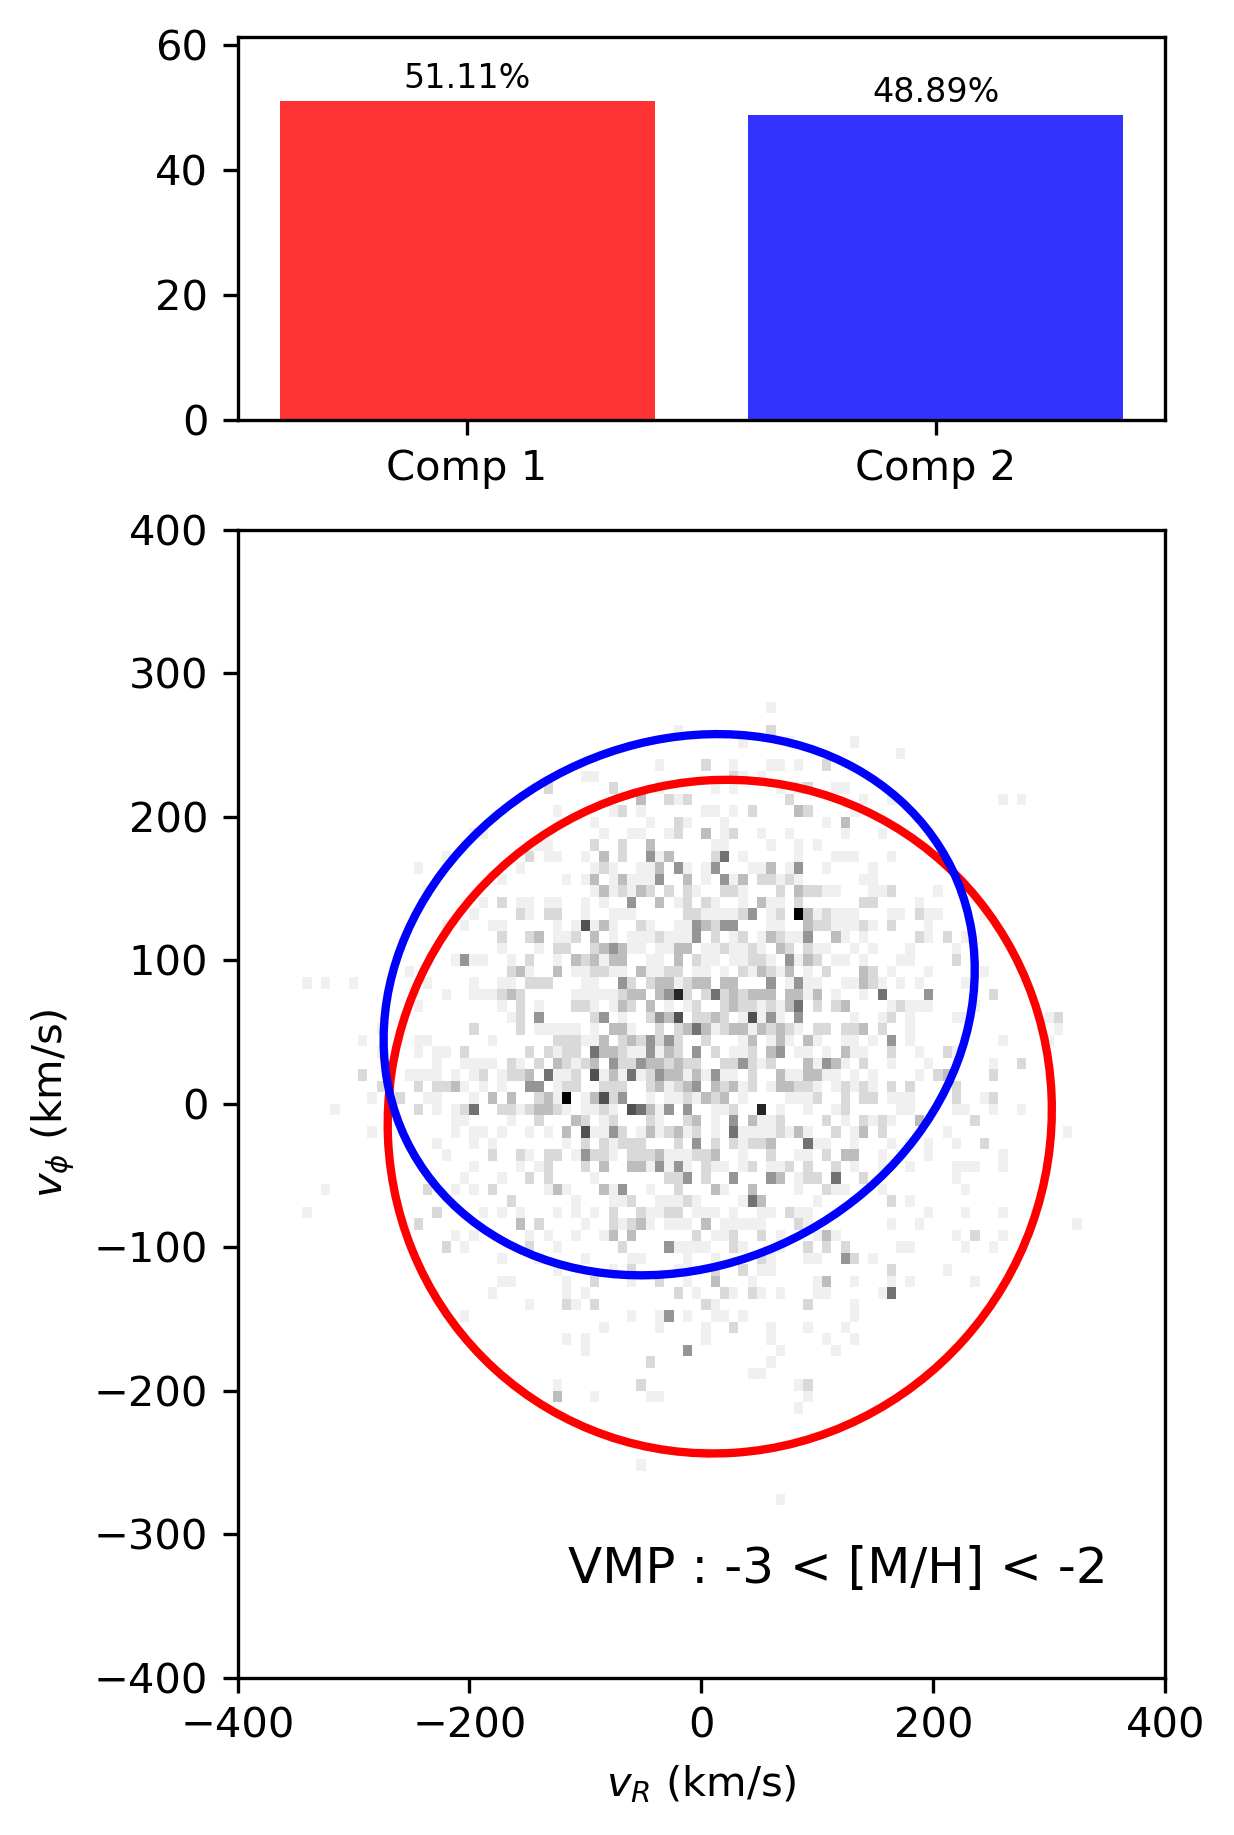
\includegraphics[width=\linewidth]{../figures/gmm_VMP.png}
    \caption{\href{https://raw.githack.com/raunaq-rai/Disentangling-the-Milky-Way-using-GMM/main/figures/VMP\_\_-3\%5BM\_H\%5D-2.html}{VMP}}
    \label{fig:gmm_vmp}
  \end{subfigure}\hfill
  \begin{subfigure}[t]{0.24\linewidth}
    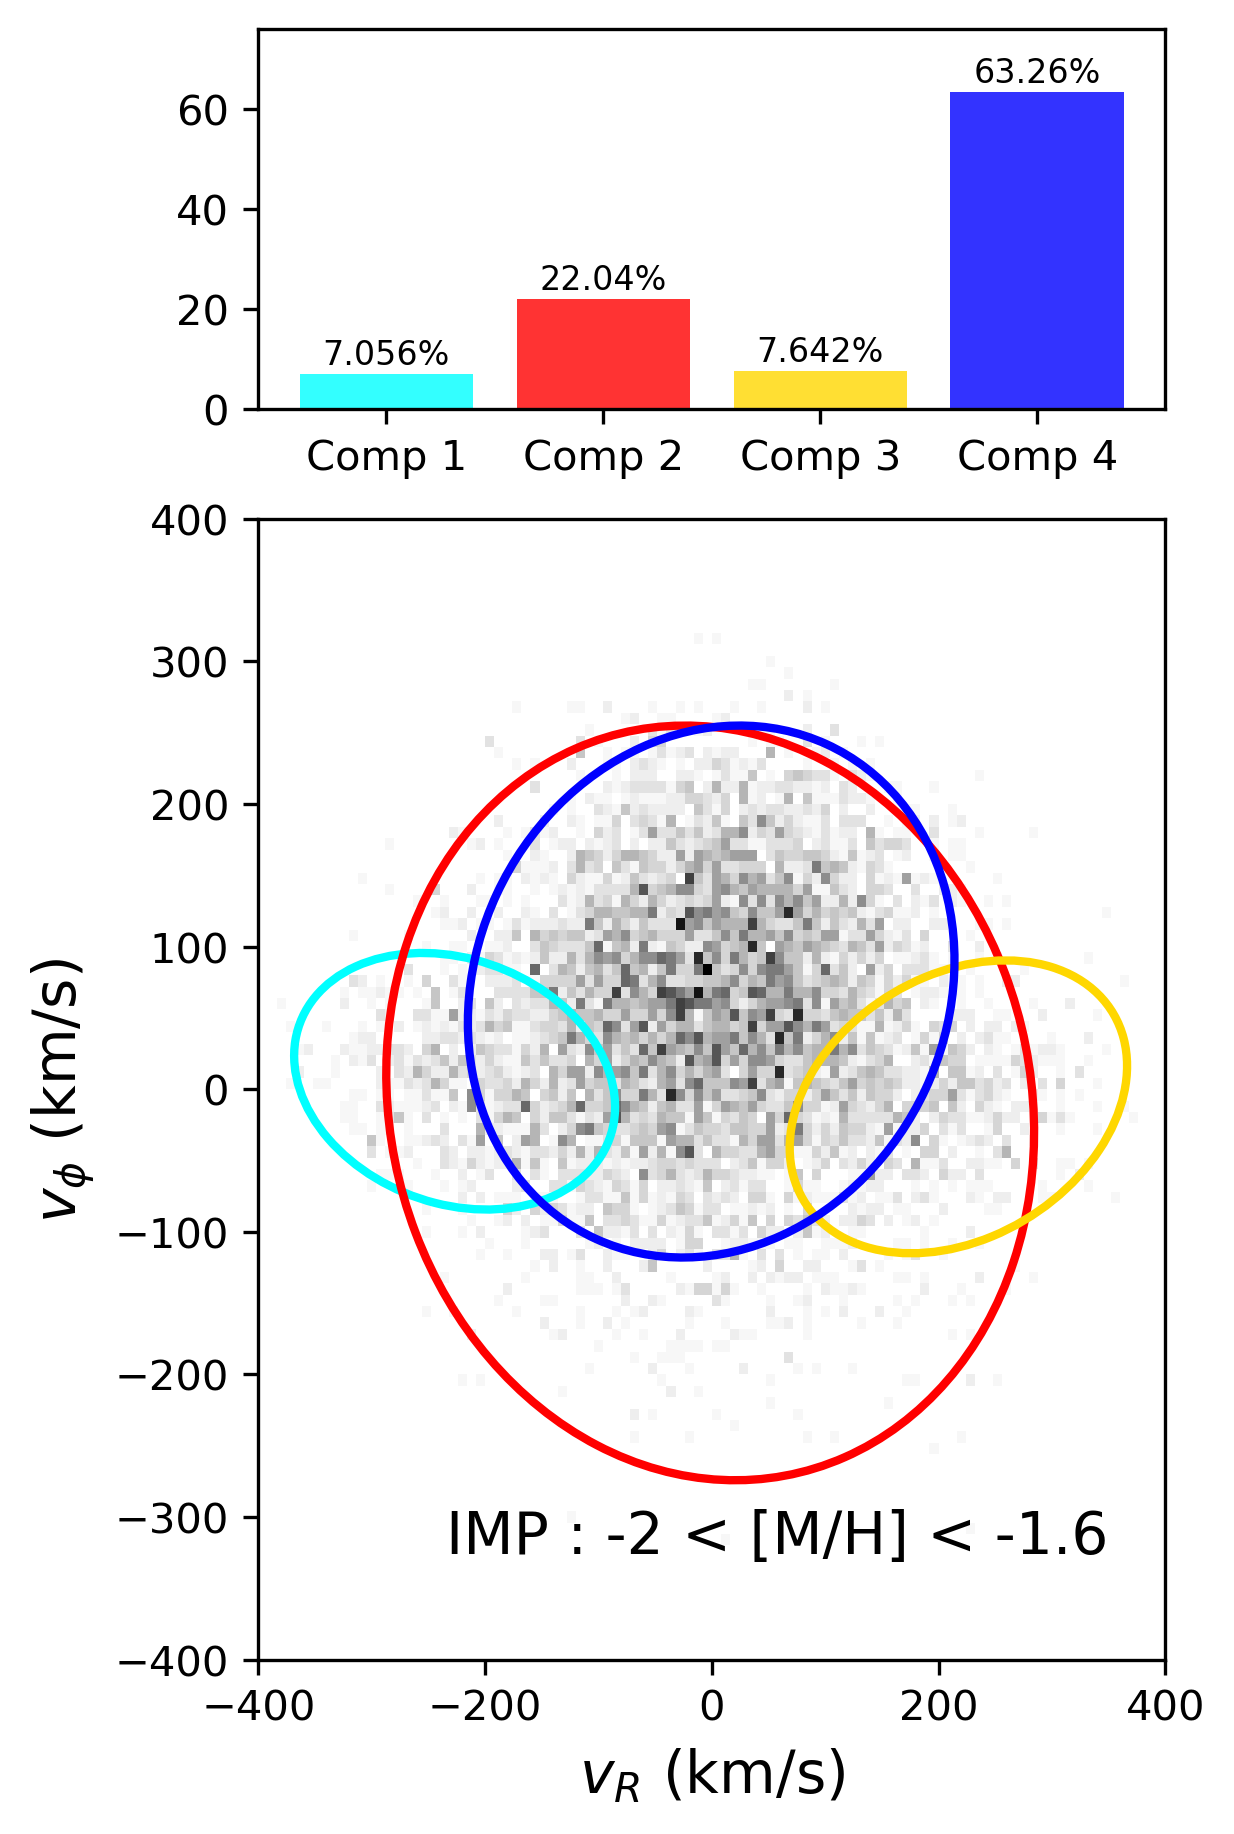
\includegraphics[width=\linewidth]{../figures/gmm_IMP.png}
    \caption{\href{https://raw.githack.com/raunaq-rai/Disentangling-the-Milky-Way-using-GMM/main/figures/IMP\_\_-2\%5BM\_H\%5D-1.6.html}{IMP}}
    \label{fig:gmm_imp}
  \end{subfigure}\hfill
  \begin{subfigure}[t]{0.24\linewidth}
    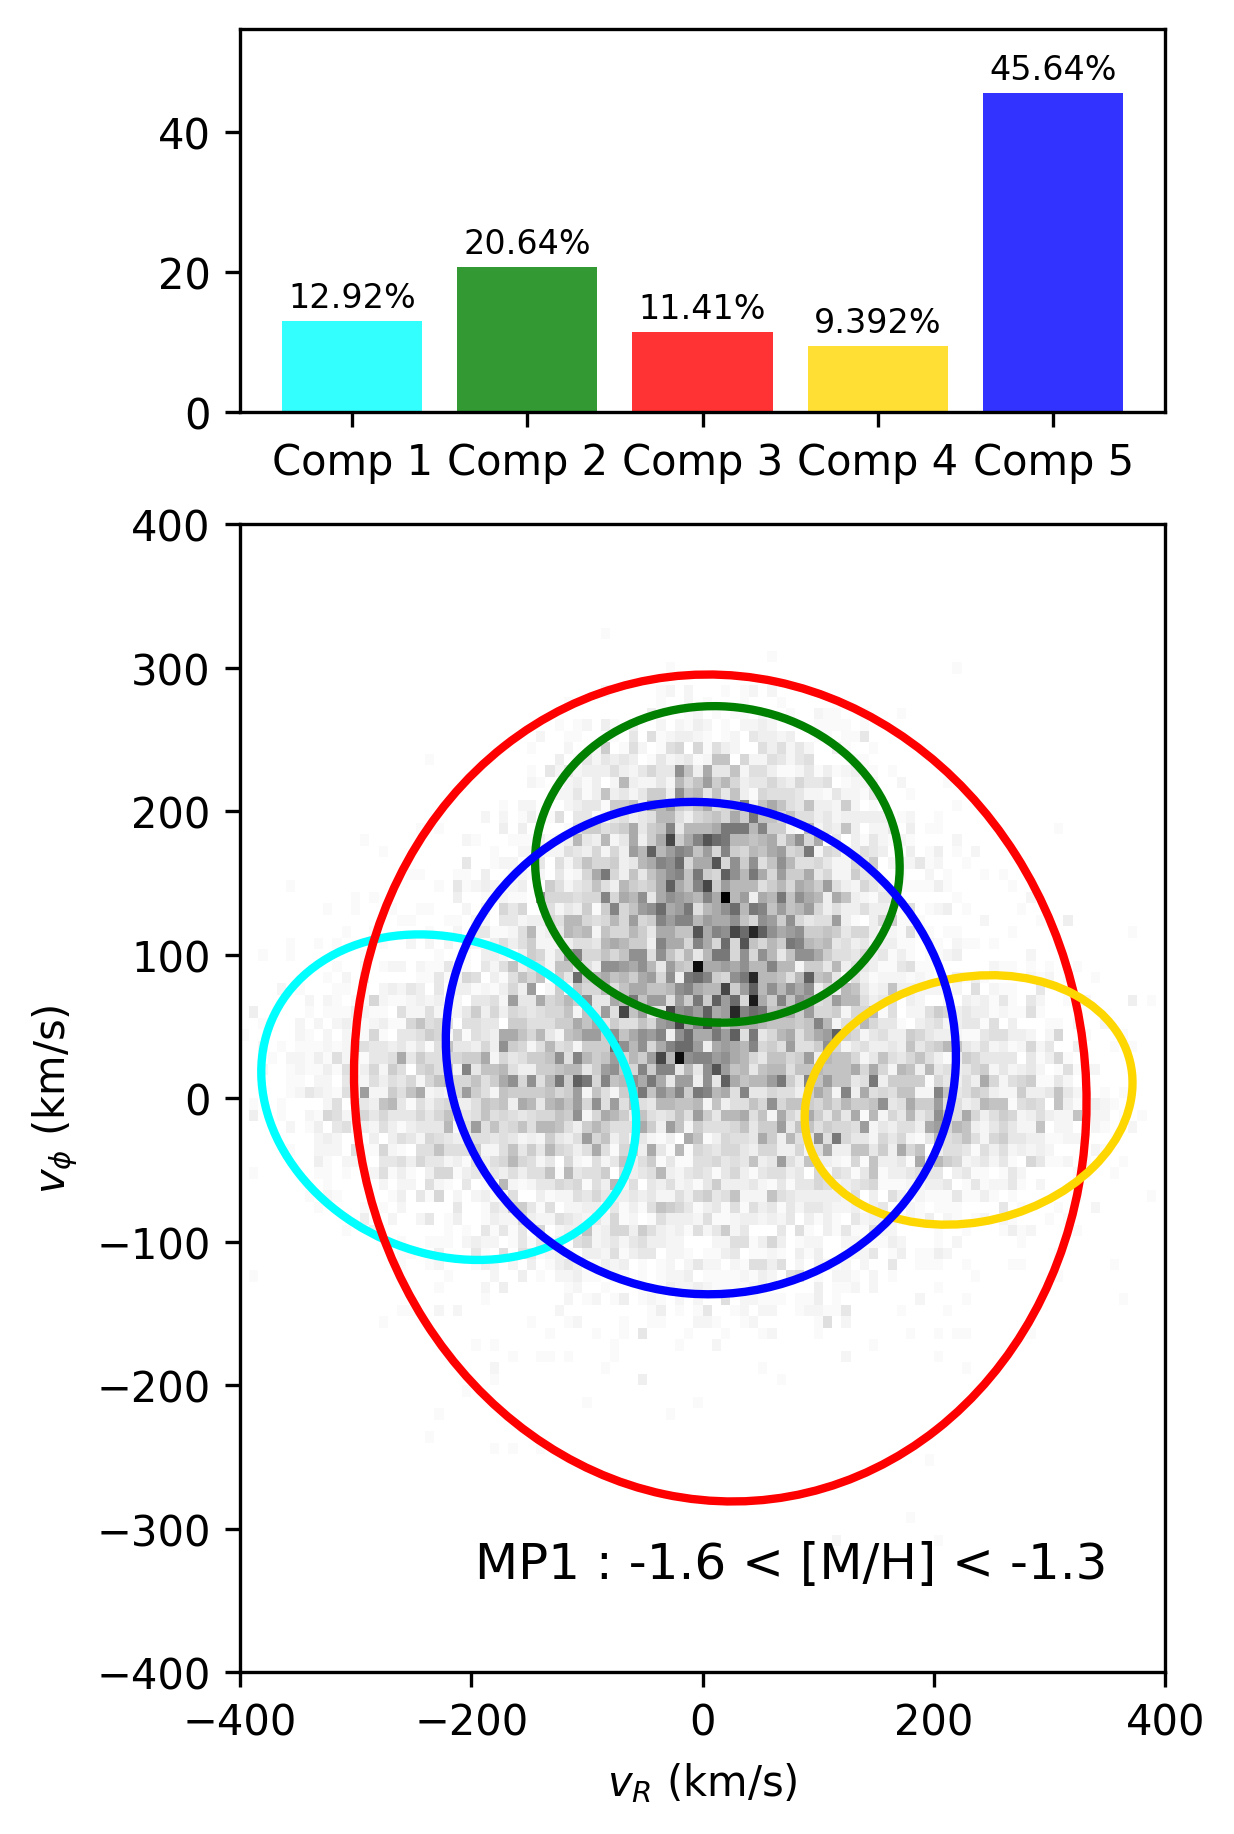
\includegraphics[width=\linewidth]{../figures/gmm_MP1.png}
    \caption{\href{https://raw.githack.com/raunaq-rai/Disentangling-the-Milky-Way-using-GMM/main/figures/MP1\_\_-1.6\%5BM\_H\%5D-1.3.html}{MP1}}
    \label{fig:gmm_mp1}
  \end{subfigure}\hfill
  \begin{subfigure}[t]{0.24\linewidth}
    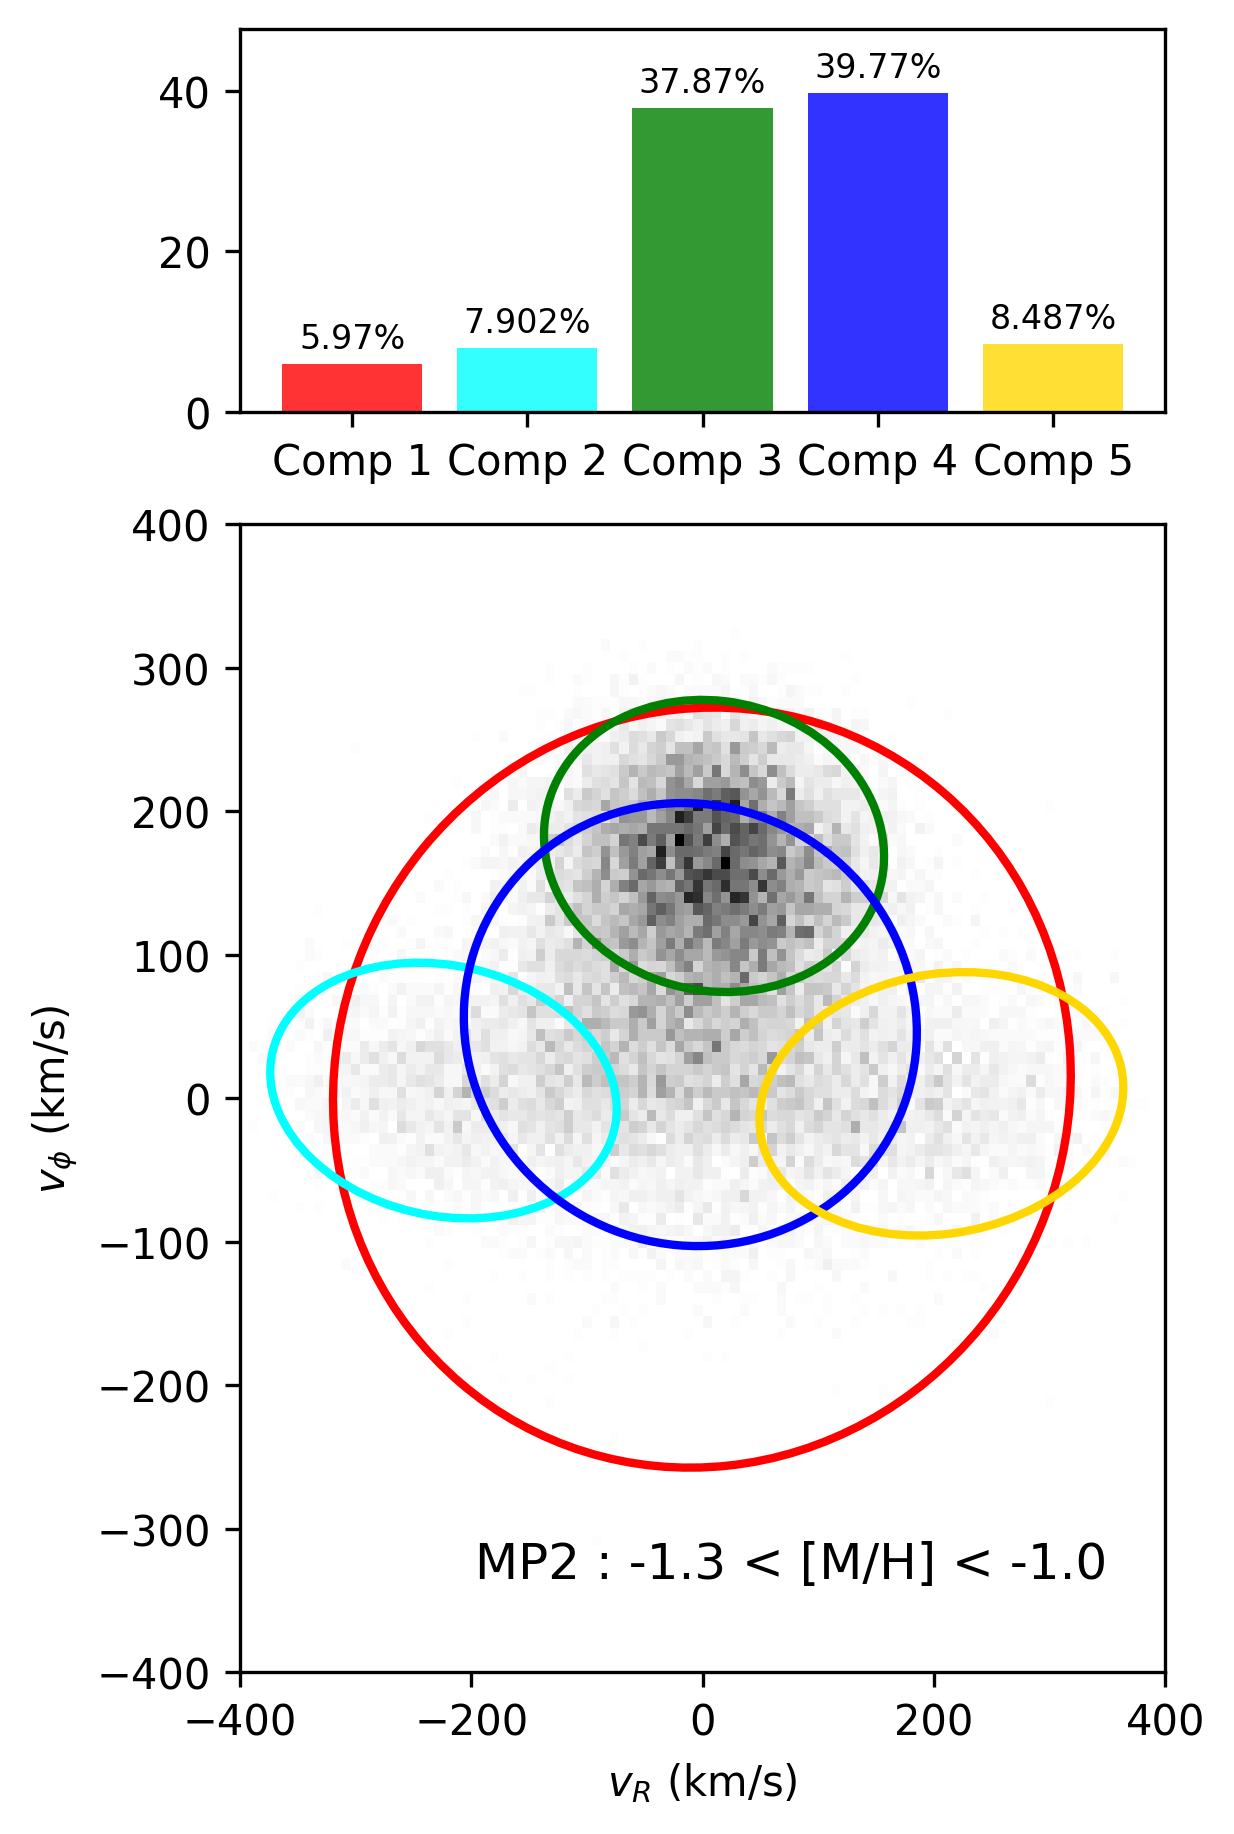
\includegraphics[width=\linewidth]{../figures/gmm_MP2.png}
    \caption{\href{https://raw.githack.com/raunaq-rai/Disentangling-the-Milky-Way-using-GMM/main/figures/MP2\_\_-1.3\%5BM\_H\%5D-1.0.html}{MP2}}
    \label{fig:gmm_mp2}
  \end{subfigure}

  \caption{XD–GMM decomposition of red giant kinematics across metallicity bins.}
  \label{fig:gmm_zhang}
\end{figure}


Below $\mathrm{[M/H]} \sim -2$, no disc-like component is detected. The kinematics are fully 
explained by two broad halo Gaussians: one stationary and one mildly prograde likely associated 
with the Aurora population~\cite{Belokurov2022}. In the intermediate metallicity bin, two 
additional highly radial, non-rotating components emerge, linked to the 
Gaia–Sausage/Enceladus (GS/E) merger~\cite{Belokurov2018}. These represent remnants of a 
major head-on collision between the Milky Way and a massive dwarf galaxy, which deposited stars 
on radial orbits and contributed significantly to the inner halo's anisotropic structure.

Disc-like rotation only emerges above $\mathrm{[M/H]} \sim -1.6$: a distinct prograde component with 
relatively low dispersion, consistent with an early thick disc is observable. 
This component strengthens with increasing metallicity, supporting a gradual buildup of 
ordered rotation as the Galaxy chemically enriched.


In the MP1 bin (around $\mathrm{[M/H]}\sim-1.5$), a thick disc begins to appear, 
rotating at $\langle v_{\phi}\rangle \approx160\ \mathrm{km\,s^{-1}}$ with $\sigma_{\phi}\approx57\ \mathrm{km\,s^{-1}}$, 
yielding $V_{\rm rot}/\sigma_{\phi}\approx2.8$ (just below the conventional “discy” threshold of $\sim3$) accounting for $\sim22\%$ of the stars. 
By the MP2 bin (higher metallicity), the disc becomes the dominant component (37.4\% by weight) and surpasses the discy criterion with 
$V_{\rm rot}/\sigma_{\phi}\approx3.5$, suggesting a well‐established, rotation‐supported structure. 

Monte Carlo residual analysis in the VMP and IMP bins detects only minor excesses, 
constraining any hidden low‐metallicity disc to at most $\sim1\%$ of the sample. Together, these diagnostics suggest the 
absence of a disc below $\mathrm{[M/H]}\sim-1.6$).  


Extending our analysis, we follow the method proposed by Viswanathan et al.~\cite{Vis2024} to separate our sample into 
high and low $\alpha$ sequences. This $\alpha$ abundance reflects star formation timescales: high $\alpha$ 
stars typically formed rapidly in intense, early starbursts, while low $\alpha$ stars 
formed more gradually over extended periods, often in lower density environments.

Figure~\ref{fig:mh_vphi_alpha} shows how these two populations differ in their kinematic evolution. 
In the high $\alpha$ branch, we observe a smooth increase in mean azimuthal velocity and a concurrent 
decrease in dispersion with increasing metallicity, indicating a gradual spin-up from a dynamically hot 
halo to a thick disc. In contrast, the low $\alpha$ population undergoes a sharper transition: 
rotation and cooling only emerge above $\mathrm{[M/H]} \sim -1.3$, consistent with a younger, thin disc origin.

\begin{figure}[H]
  \centering
  \begin{subfigure}[t]{0.48\linewidth}
    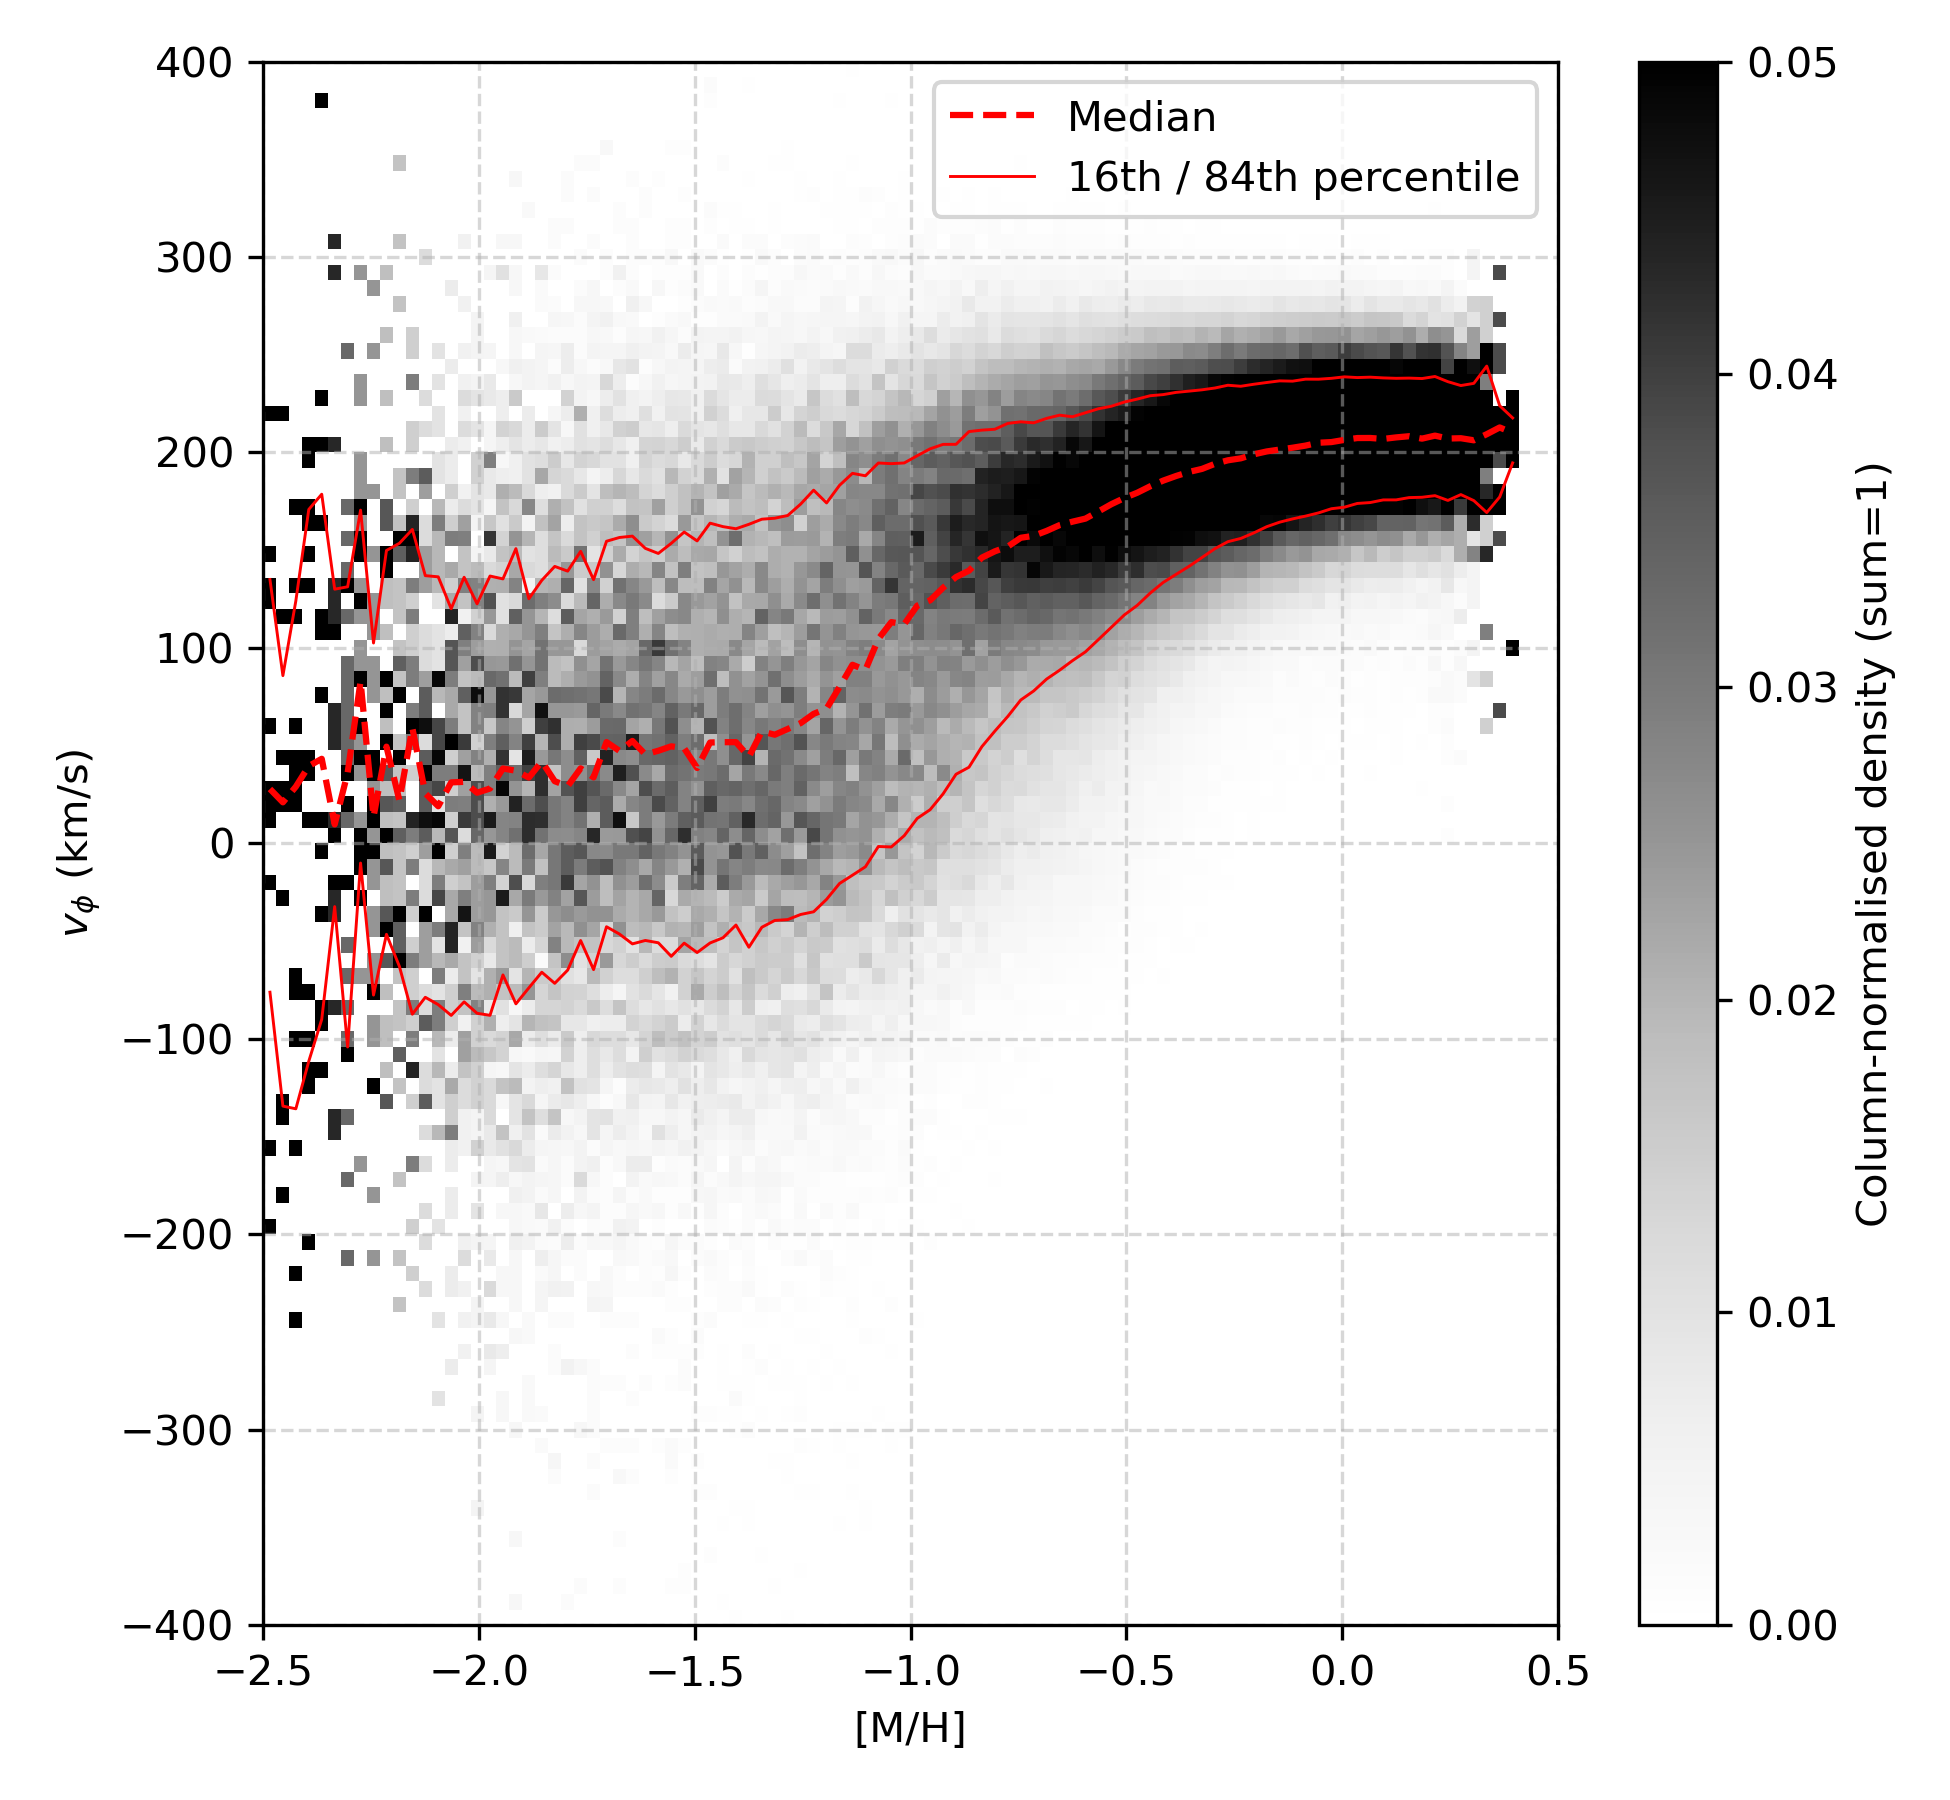
\includegraphics[width=\linewidth]{../figures/vis_mh_vphi_high_alpha.png}
    \caption{High $\alpha$ stars}
  \end{subfigure}
  \hfill
  \begin{subfigure}[t]{0.48\linewidth}
    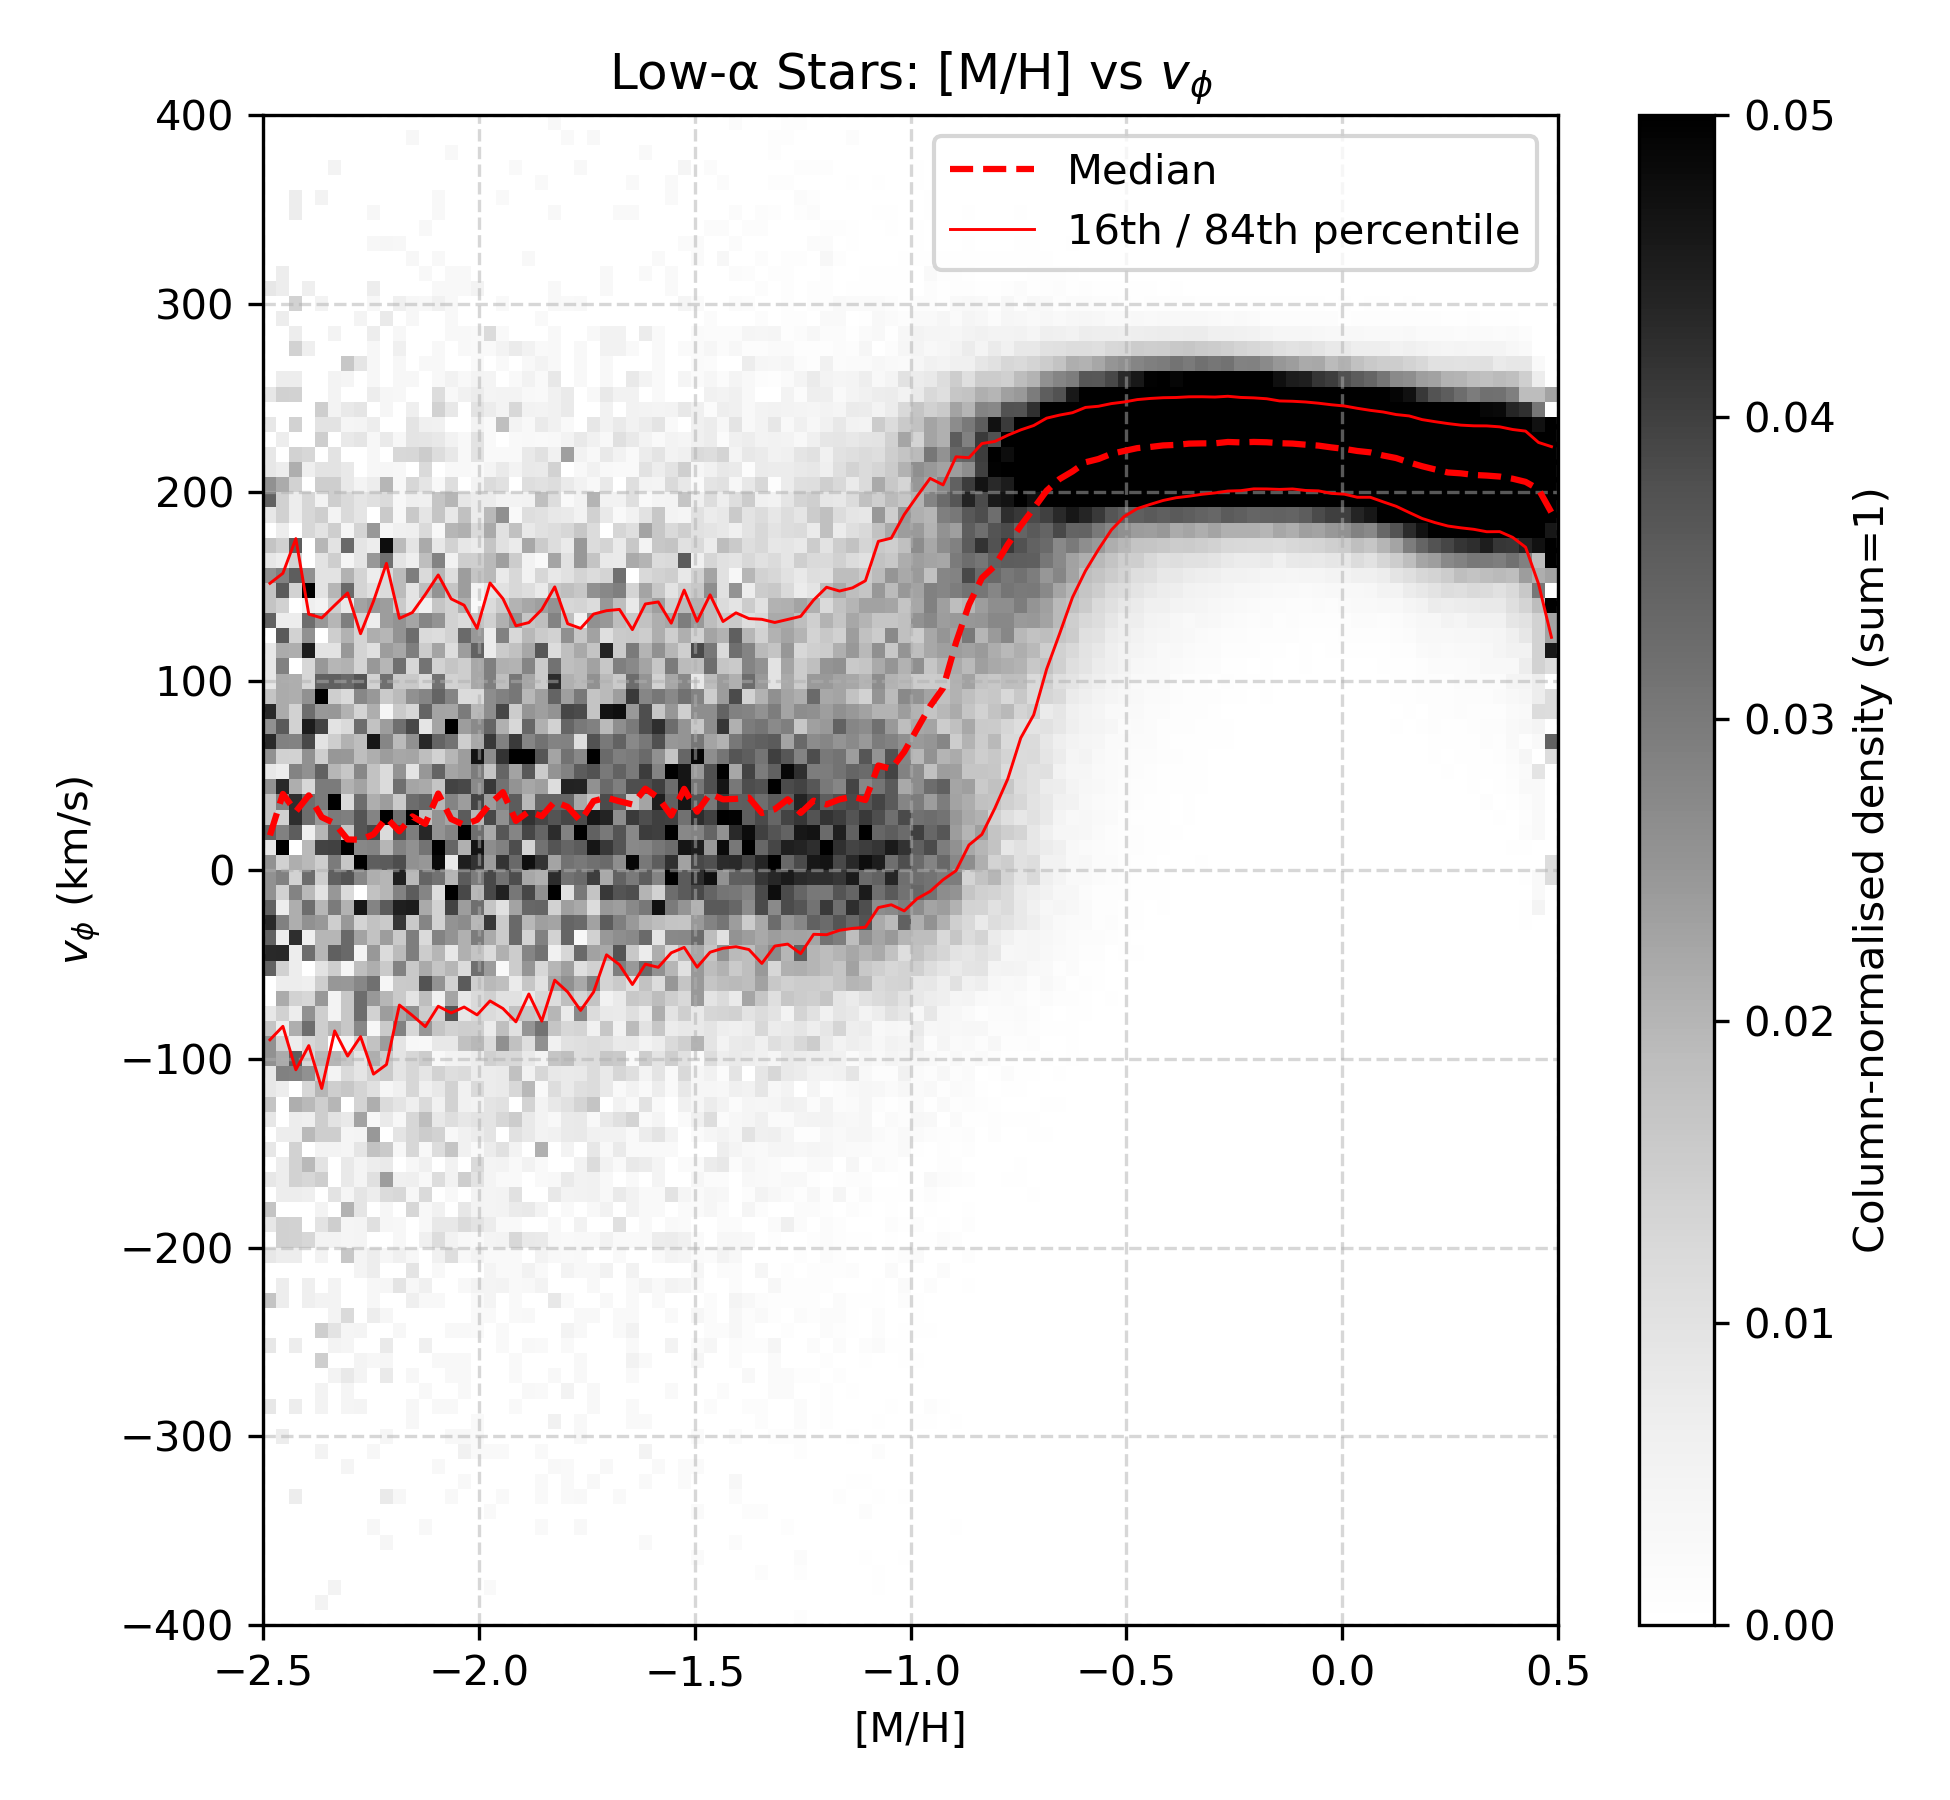
\includegraphics[width=\linewidth]{../figures/vis_mh_vphi_low_alpha.png}
    \caption{Low $\alpha$ stars}
  \end{subfigure}
  \caption{Median $v_\phi$ and dispersion vs.\ metallicity, split by $\alpha$-sequence.}
  \label{fig:mh_vphi_alpha}
\end{figure}

We applied XD–GMMs to the high‐ and low‐$\alpha$ sequences separately (Figure~\ref{fig:gmm_alpha_bins}).  
In the \textit{high‐$\alpha$} track, only a non-rotating halo is present at $\mathrm{[M/H]}\!\lesssim\!-2$.  
A thick-disc Gaussian first appears at $-1.6\!\lesssim\!\mathrm{[M/H]}\!\lesssim\!-1.3$ (31 \% by weight), rotating at $\langle v_{\phi}\rangle\!\approx\!148\ \mathrm{km\,s^{-1}}$ with $\sigma_{\phi}\!\approx\!63\ \mathrm{km\,s^{-1}}$ ($V_{\rm rot}/\sigma_{\phi}\!\approx\!2.4$).  
By $-1.3\!<\!\mathrm{[M/H]}\!<\!-1.0$ it grows to 52 \% and $V_{\rm rot}/\sigma_{\phi}\!\approx\!2.8$, charting the gradual build-up of the thick disc from $\mathrm{[M/H]}\!\sim\!-1.6$.

In the \textit{low‐$\alpha$} branch no disc is seen until $-1.3\!<\!\mathrm{[M/H]}\!<\!-1.0$, where a thin, cold component (25 \%) emerges abruptly with $\langle v_{\phi}\rangle\!\approx\!183\ \mathrm{km\,s^{-1}}$, $\sigma_{\phi}\!\approx\!48\ \mathrm{km\,s^{-1}}$ and $V_{\rm rot}/\sigma_{\phi}\!\approx\!3.8$—well above the discy threshold of~3—implying a later, rapid thin-disc formation.

GS/E-like radial Gaussians appear in both sequences, probably due to misclassified $\alpha$-poor debris, underscoring the need for robust chemical labelling.  
Overall, the high-$\alpha$ thick disc assembled earlier and gradually (\mbox{$\mathrm{[M/H]}\!\gtrsim\!-1.6$}), while the low-$\alpha$ thin disc formed later and swiftly (\mbox{$\mathrm{[M/H]}\!\gtrsim\!-1.3$}).


\begin{figure}[H]
  \centering
  % Row 1
  \begin{subfigure}[t]{0.24\linewidth}
    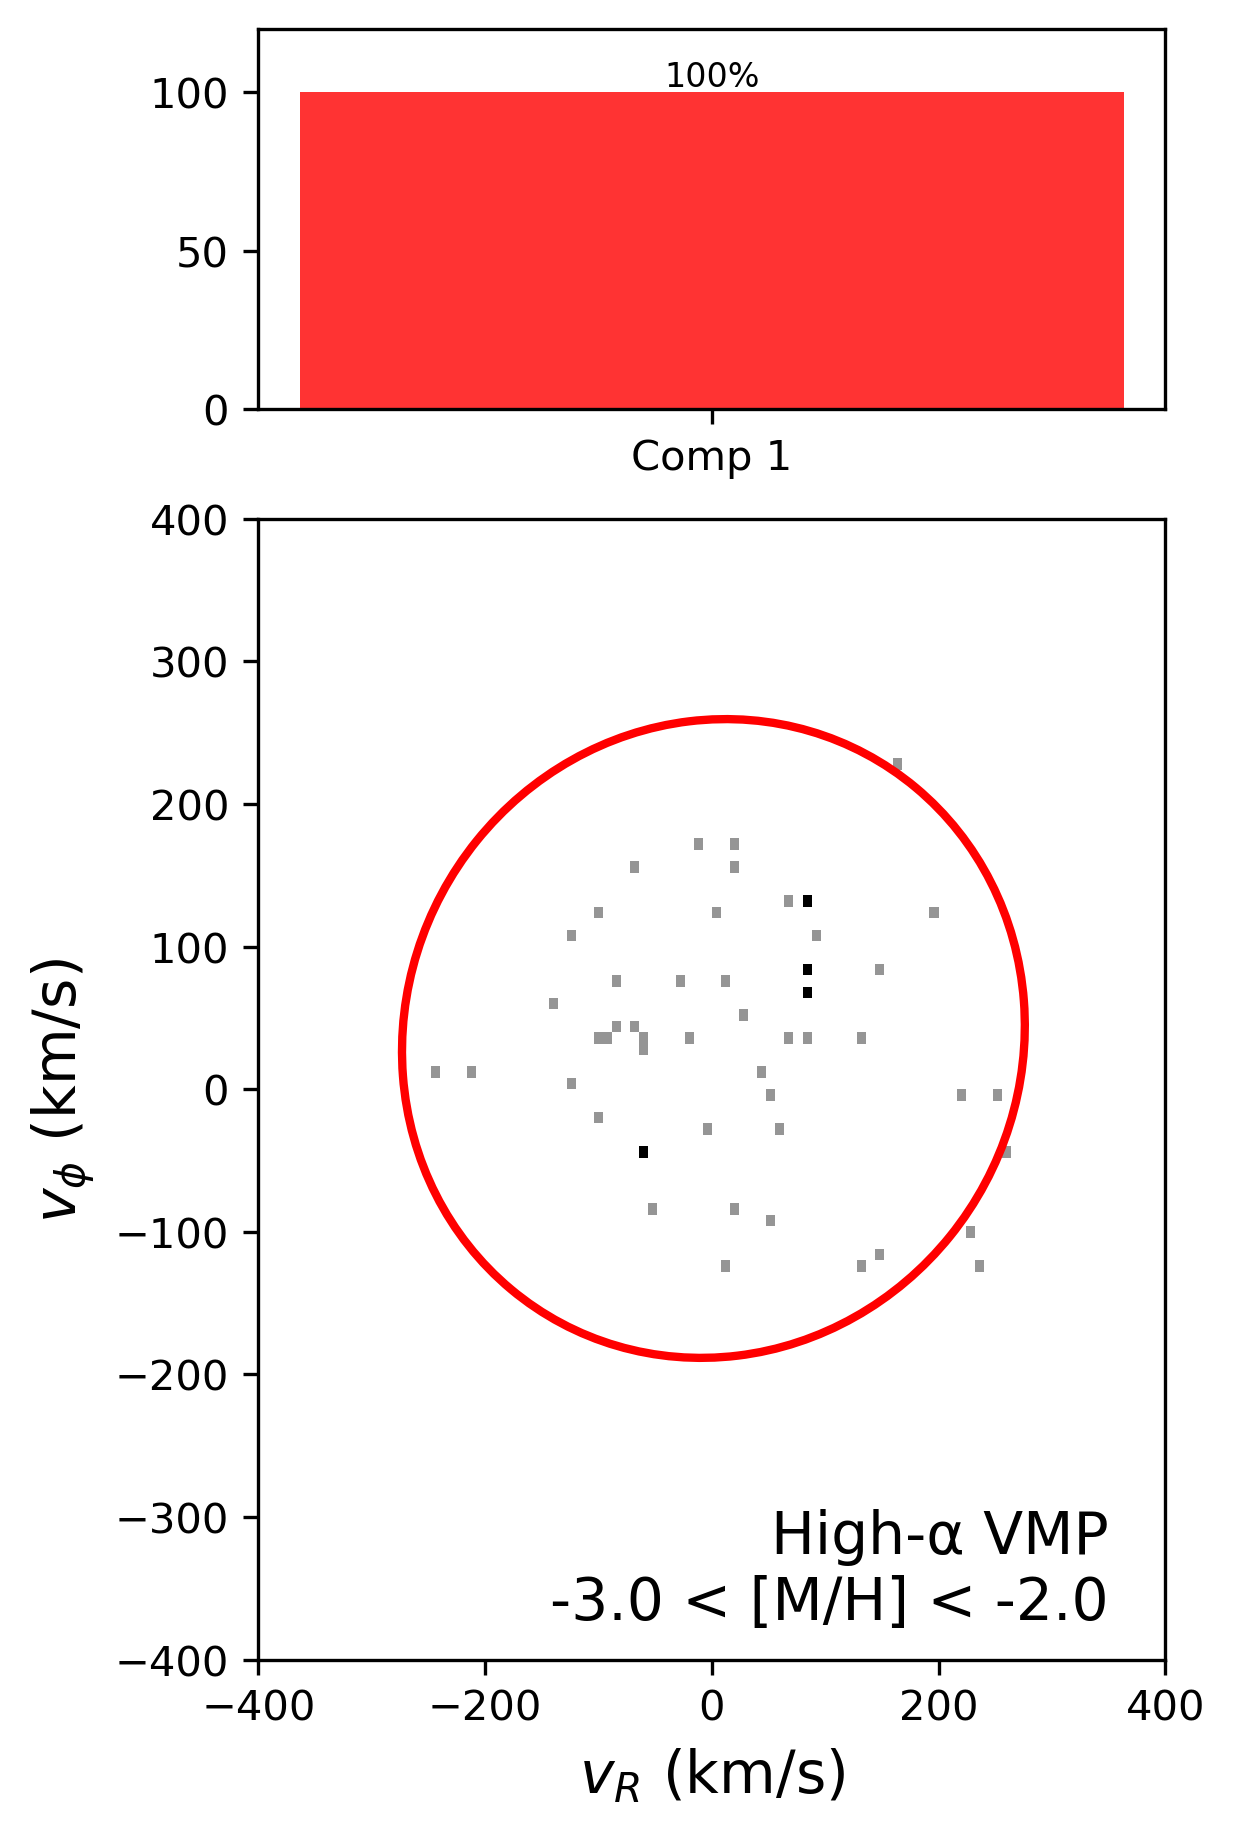
\includegraphics[width=\linewidth]{../figures/gmm_vmp_high_alpha_k1.png}
    \caption{\href{https://raw.githack.com/raunaq-rai/Disentangling-the-Milky-Way-using-GMM/main/figures/VMP\_high\_\_\_-3\%5BM\_H\%5D-2.html}{VMP $\alpha_{\mathrm{high}}$}}
    \label{fig:vmp_hi}
  \end{subfigure}\hfill
  \begin{subfigure}[t]{0.24\linewidth}
    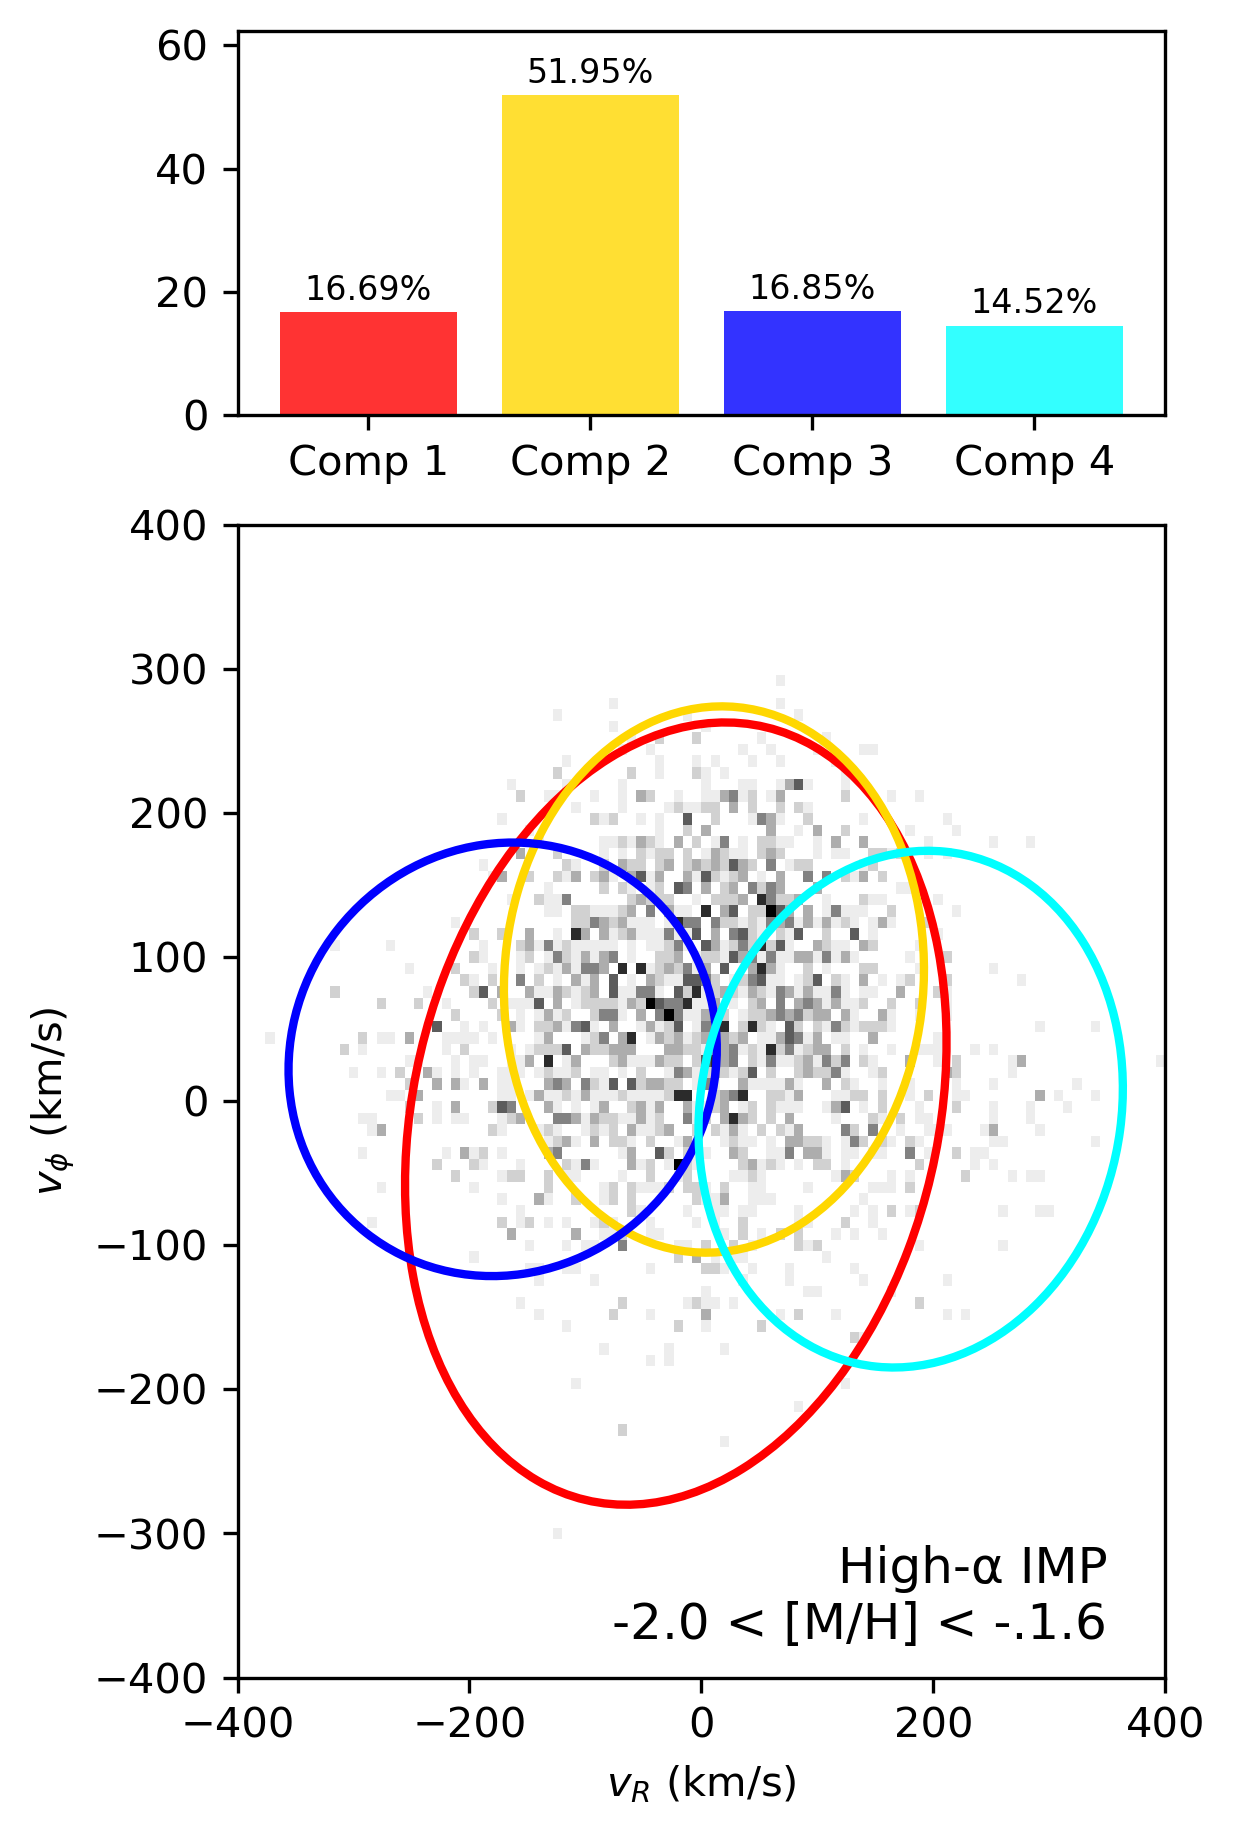
\includegraphics[width=\linewidth]{../figures/gmm_imp_high_alpha_k4.png}
    \caption{\href{https://raw.githack.com/raunaq-rai/Disentangling-the-Milky-Way-using-GMM/main/figures/IMP\_high\_\_\_-2\%5BM\_H\%5D-1.6.html}{IMP $\alpha_{\mathrm{high}}$}}
    \label{fig:imp_hi}
  \end{subfigure}\hfill
  \begin{subfigure}[t]{0.24\linewidth}
    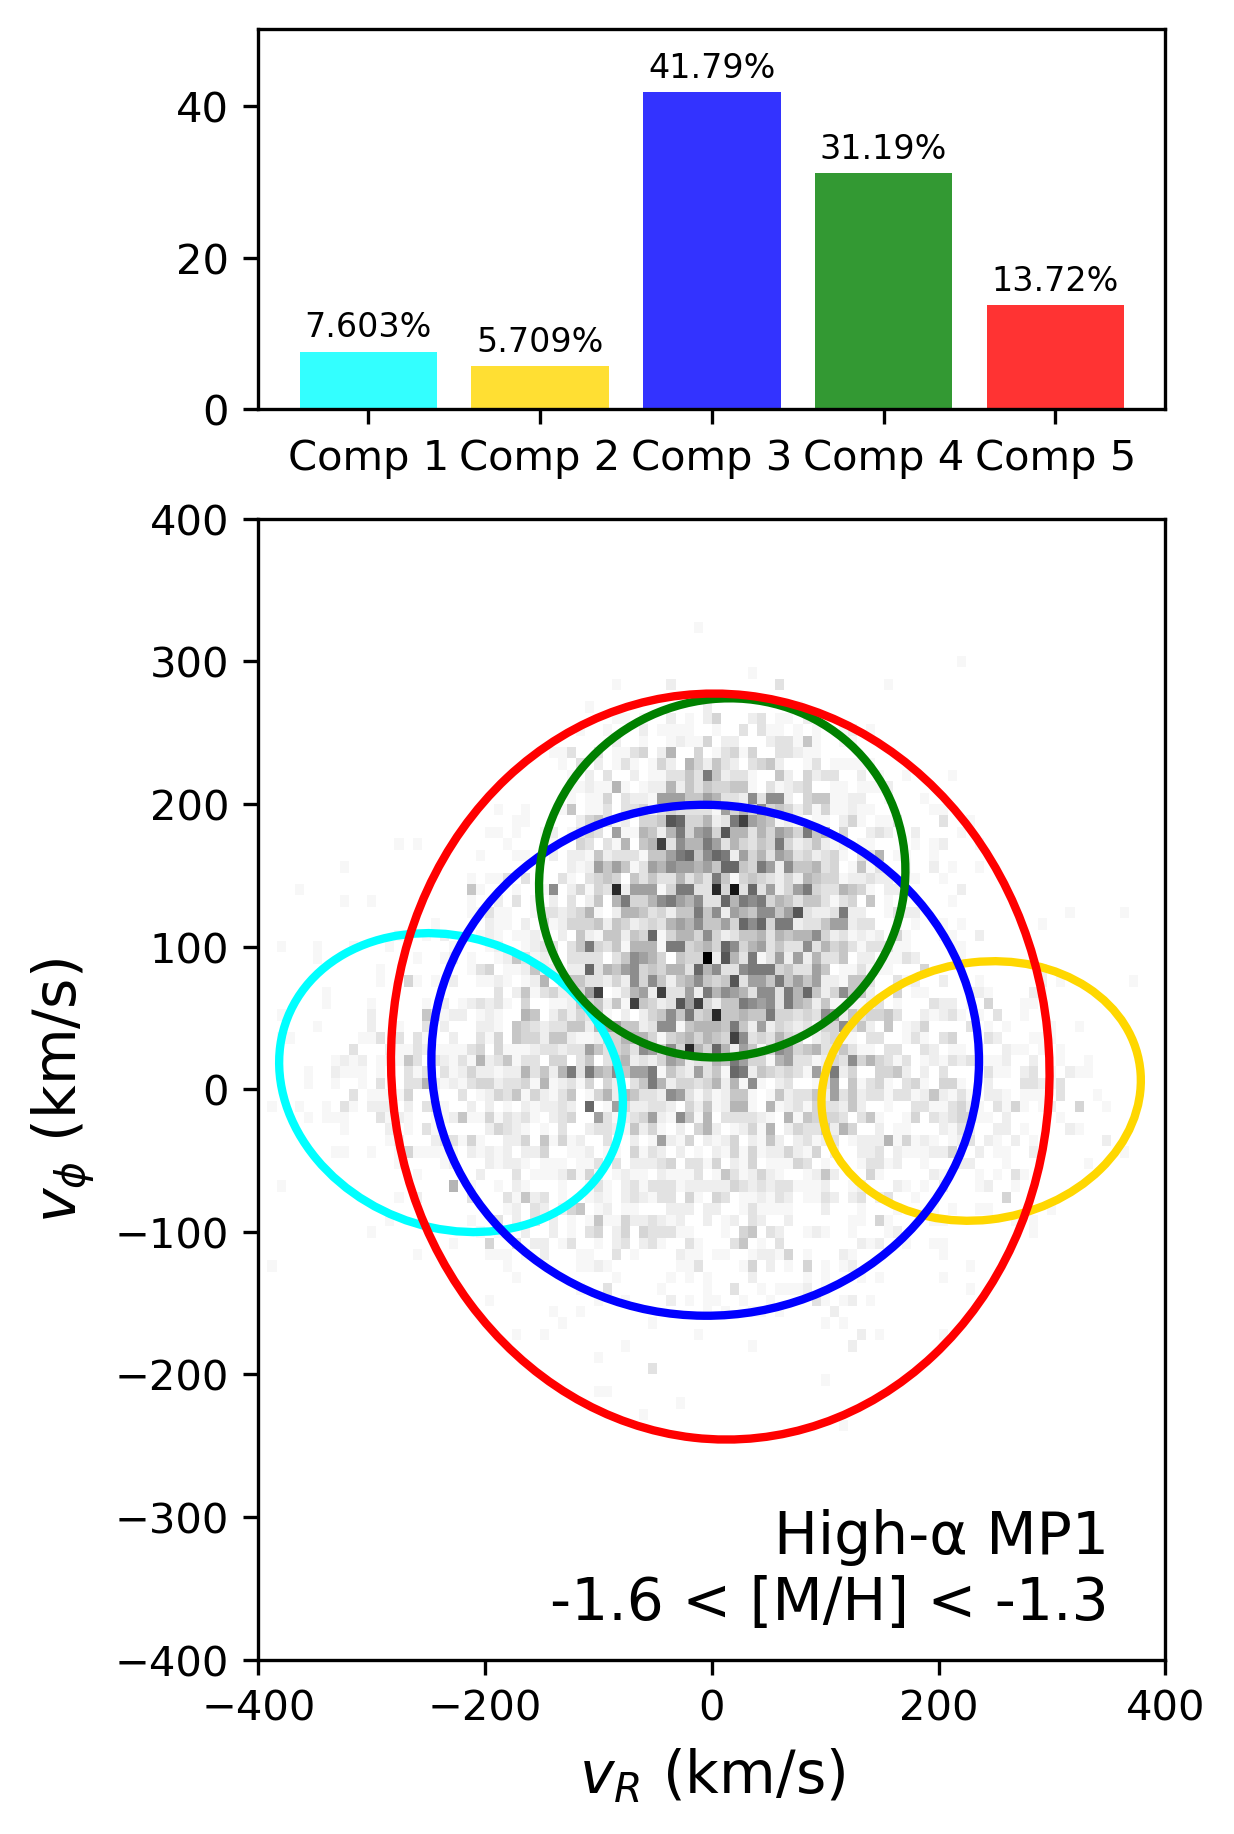
\includegraphics[width=\linewidth]{../figures/gmm_mp1_high_alpha_k5.png}
    \caption{\href{https://raw.githack.com/raunaq-rai/Disentangling-the-Milky-Way-using-GMM/main/figures/MP1\_high\_\_\_-1.6\%5BM\_H\%5D-1.3.html}{MP1 $\alpha_{\mathrm{high}}$}}
    \label{fig:mp1_hi}
  \end{subfigure}\hfill
  \begin{subfigure}[t]{0.24\linewidth}
    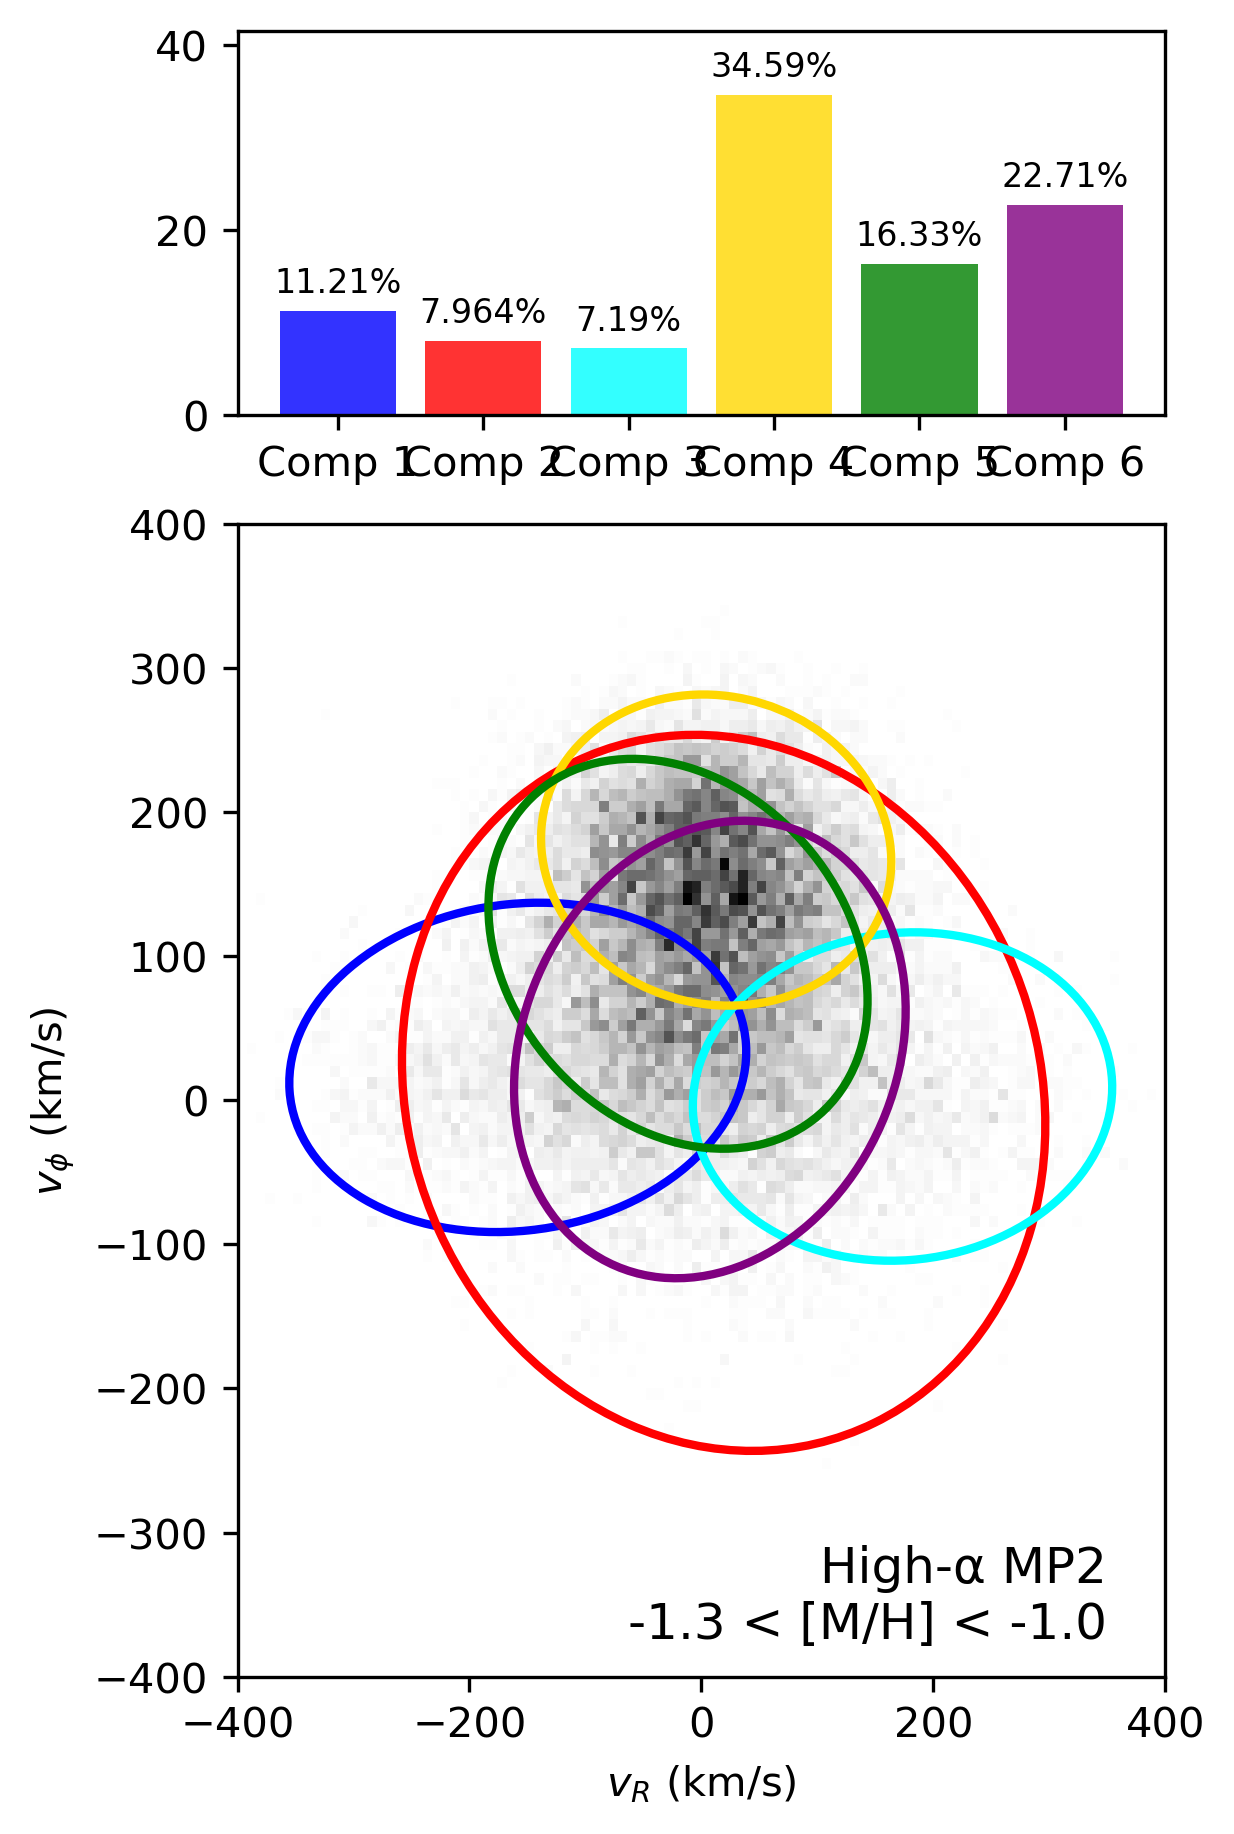
\includegraphics[width=\linewidth]{../figures/gmm_mp2_high_alpha_k6.png}
    \caption{\href{https://raw.githack.com/raunaq-rai/Disentangling-the-Milky-Way-using-GMM/main/figures/MP2\_high\_\_\_-1.3\%5BM\_H\%5D-1.0.html}{MP2 $\alpha_{\mathrm{high}}$}}
    \label{fig:mp2_hi}
  \end{subfigure}

  \vspace{0.5em}

  % Row 2: low-α (manual escapes)
  \begin{subfigure}[t]{0.24\linewidth}
    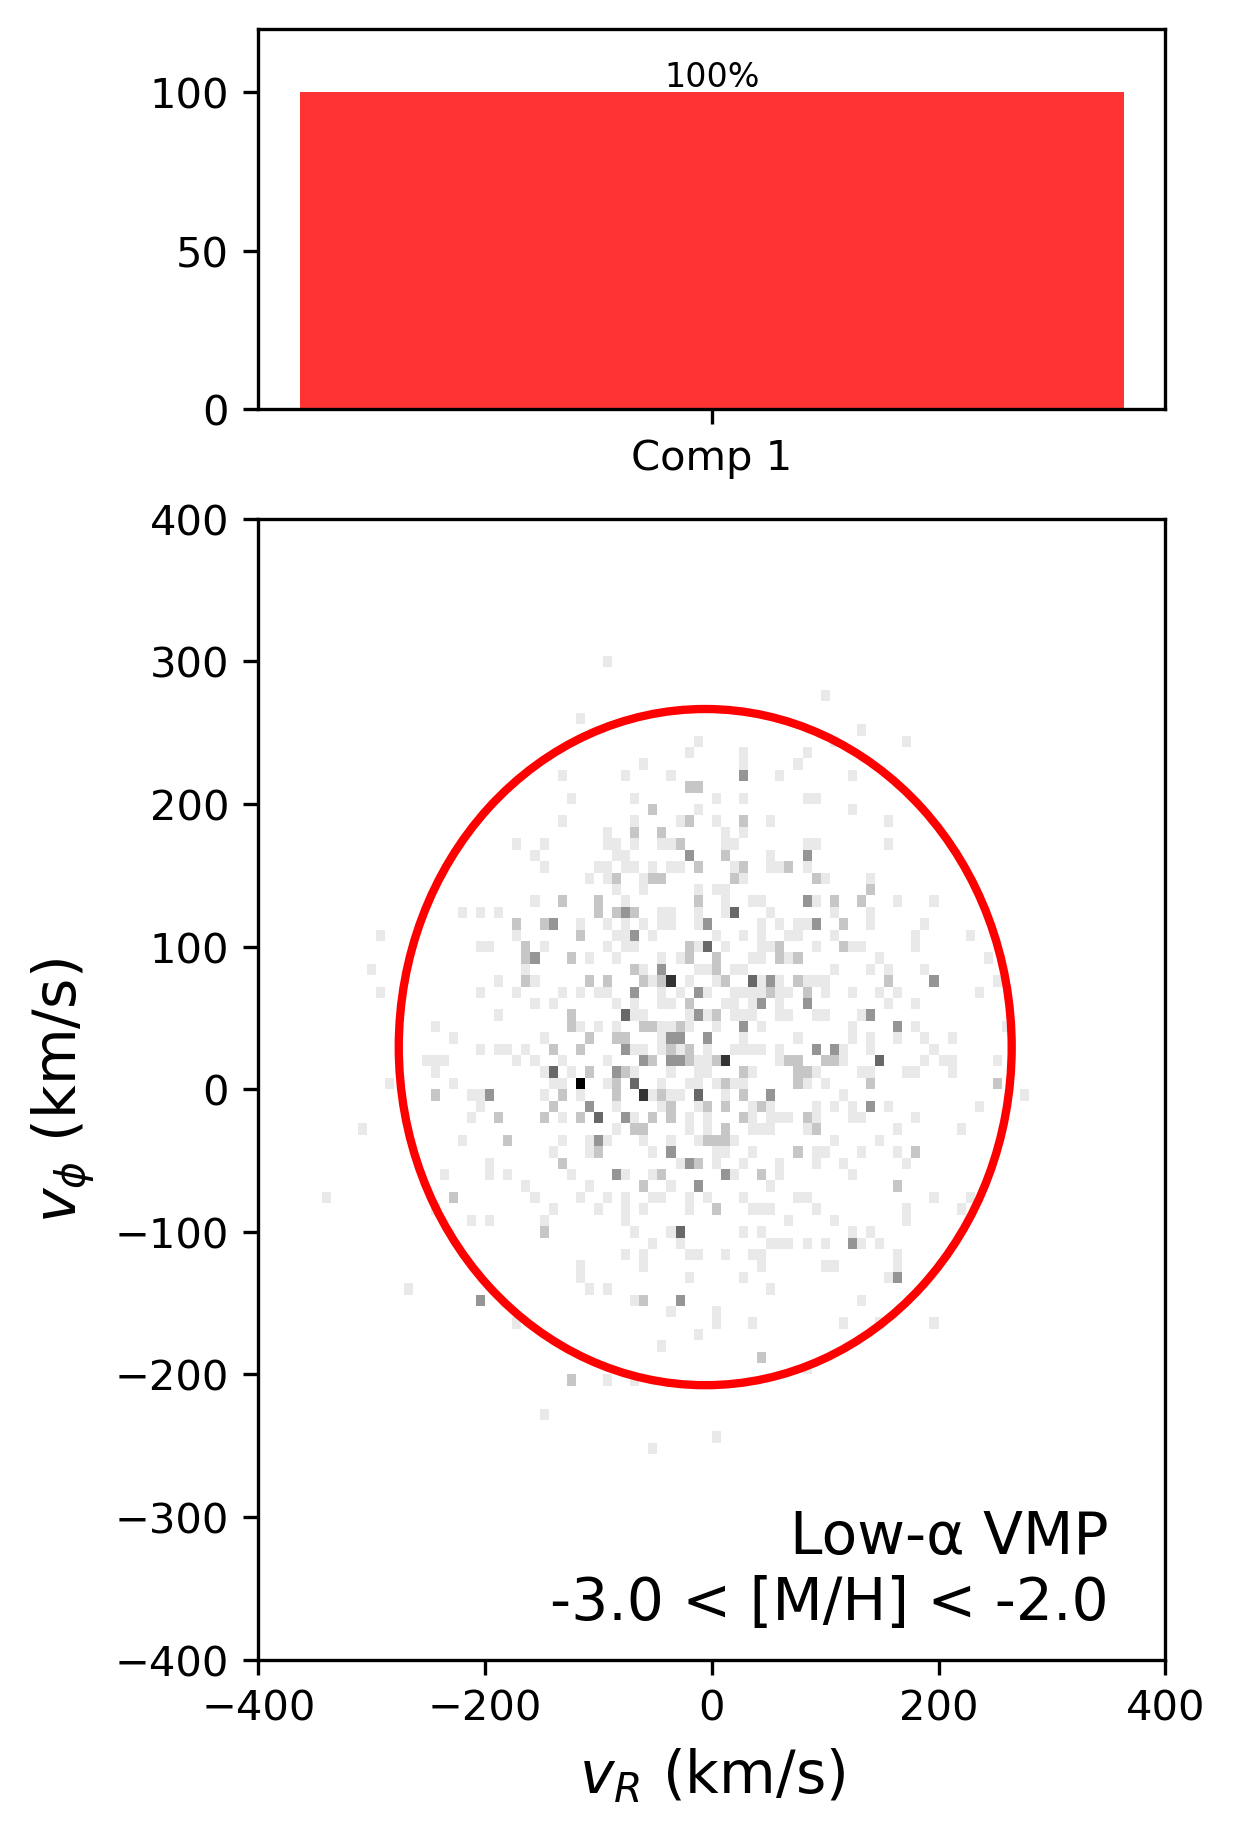
\includegraphics[width=\linewidth]{../figures/gmm_vmp_low_alpha_k1.png}
    \caption{\href{https://raw.githack.com/raunaq-rai/Disentangling-the-Milky-Way-using-GMM/main/figures/VMP\_low\_\_\_\_-3\%5BM\_H\%5D-2.html}{VMP $\alpha_{\mathrm{low}}$}}
    \label{fig:low_vmp}
  \end{subfigure}\hfill
  \begin{subfigure}[t]{0.24\linewidth}
    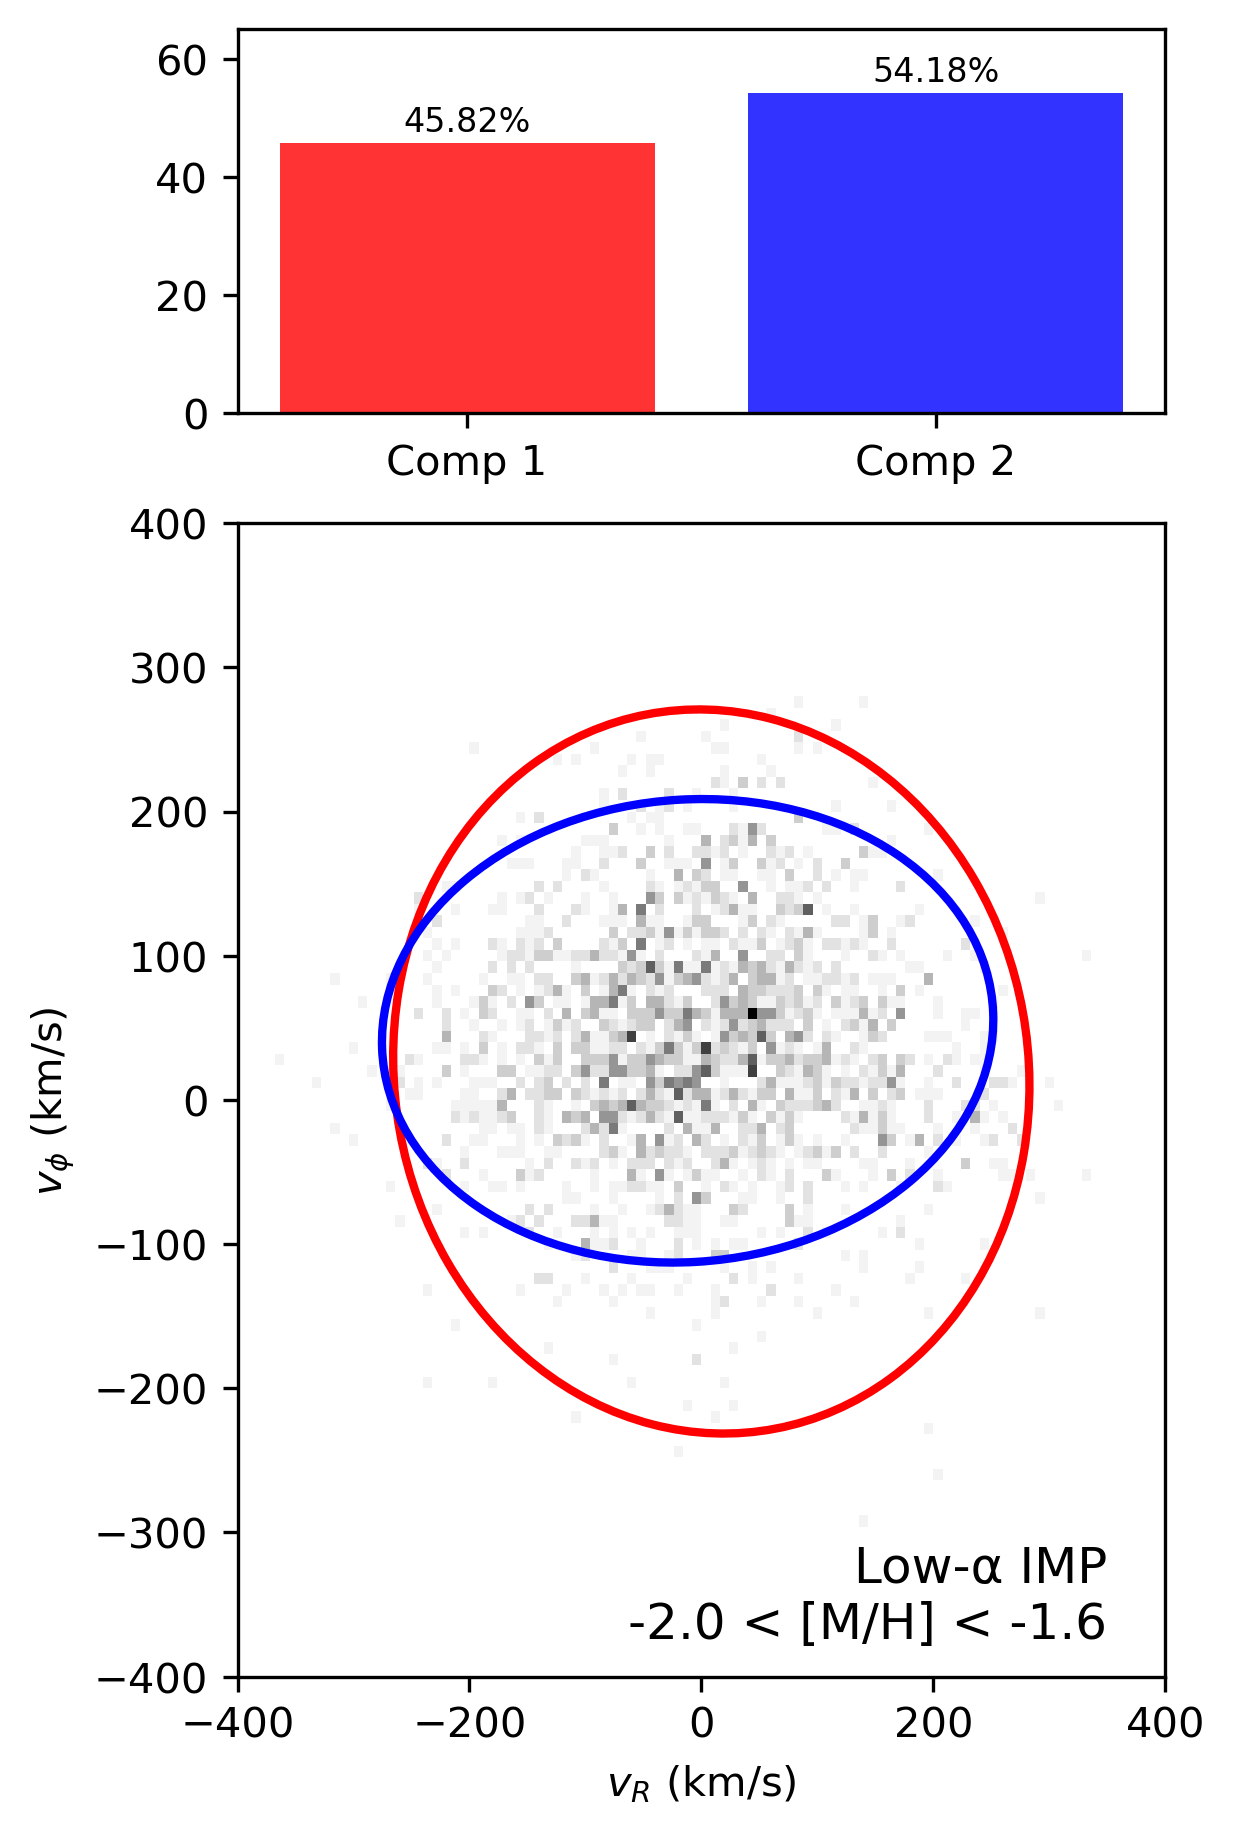
\includegraphics[width=\linewidth]{../figures/gmm_imp_low_alpha_k2.png}
    \caption{\href{https://raw.githack.com/raunaq-rai/Disentangling-the-Milky-Way-using-GMM/main/figures/IMP\_low\_\_\_\_-2\%5BM\_H\%5D-1.6.html}{IMP $\alpha_{\mathrm{low}}$}}
    \label{fig:low_imp}
  \end{subfigure}\hfill
  \begin{subfigure}[t]{0.24\linewidth}
    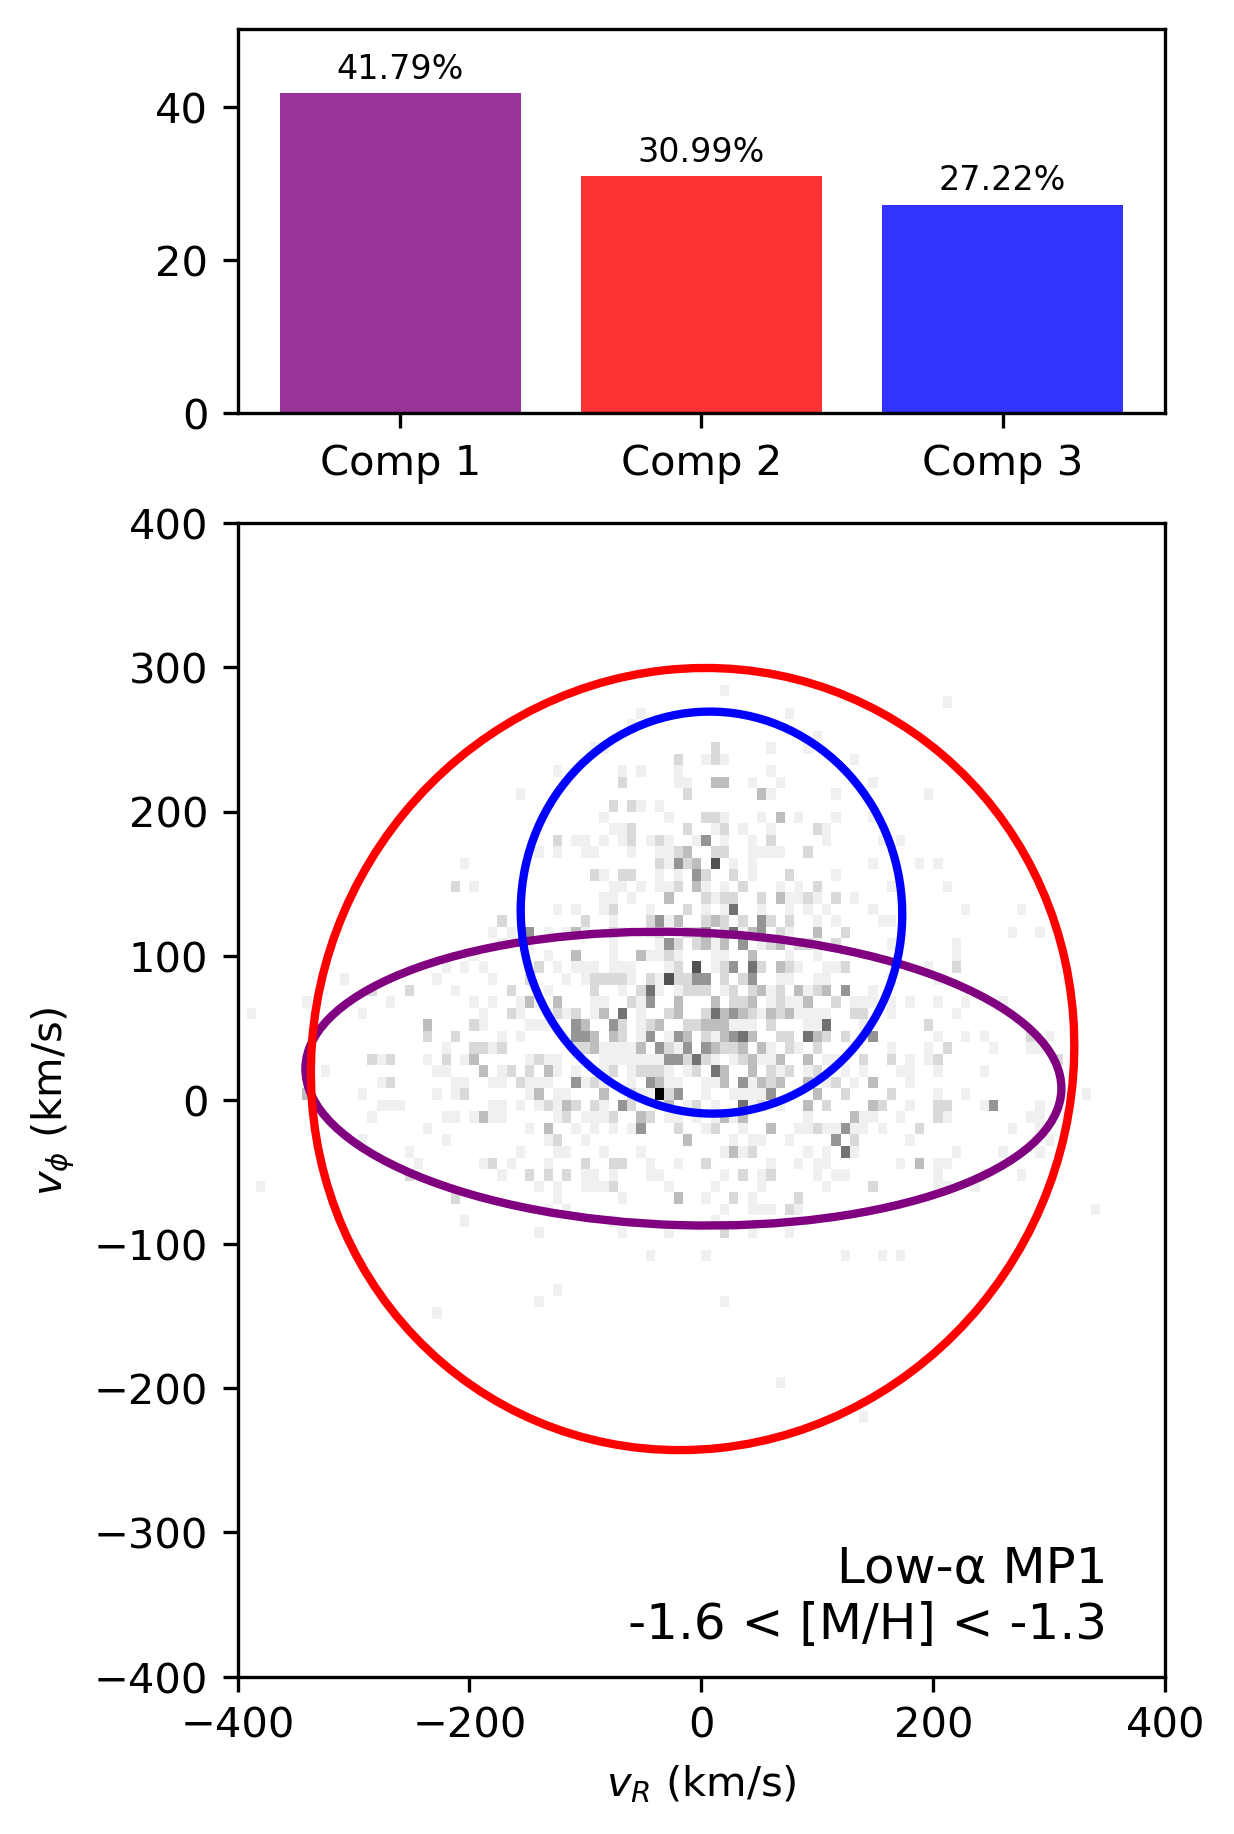
\includegraphics[width=\linewidth]{../figures/gmm_mp1_low_alpha_k4.png}
    \caption{\href{https://raw.githack.com/raunaq-rai/Disentangling-the-Milky-Way-using-GMM/main/figures/MP1\_low\_\_\_\_-1.6\%5BM\_H\%5D-1.3.html}{MP1 $\alpha_{\mathrm{low}}$}}
    \label{fig:low_mp1}
  \end{subfigure}\hfill
  \begin{subfigure}[t]{0.24\linewidth}
    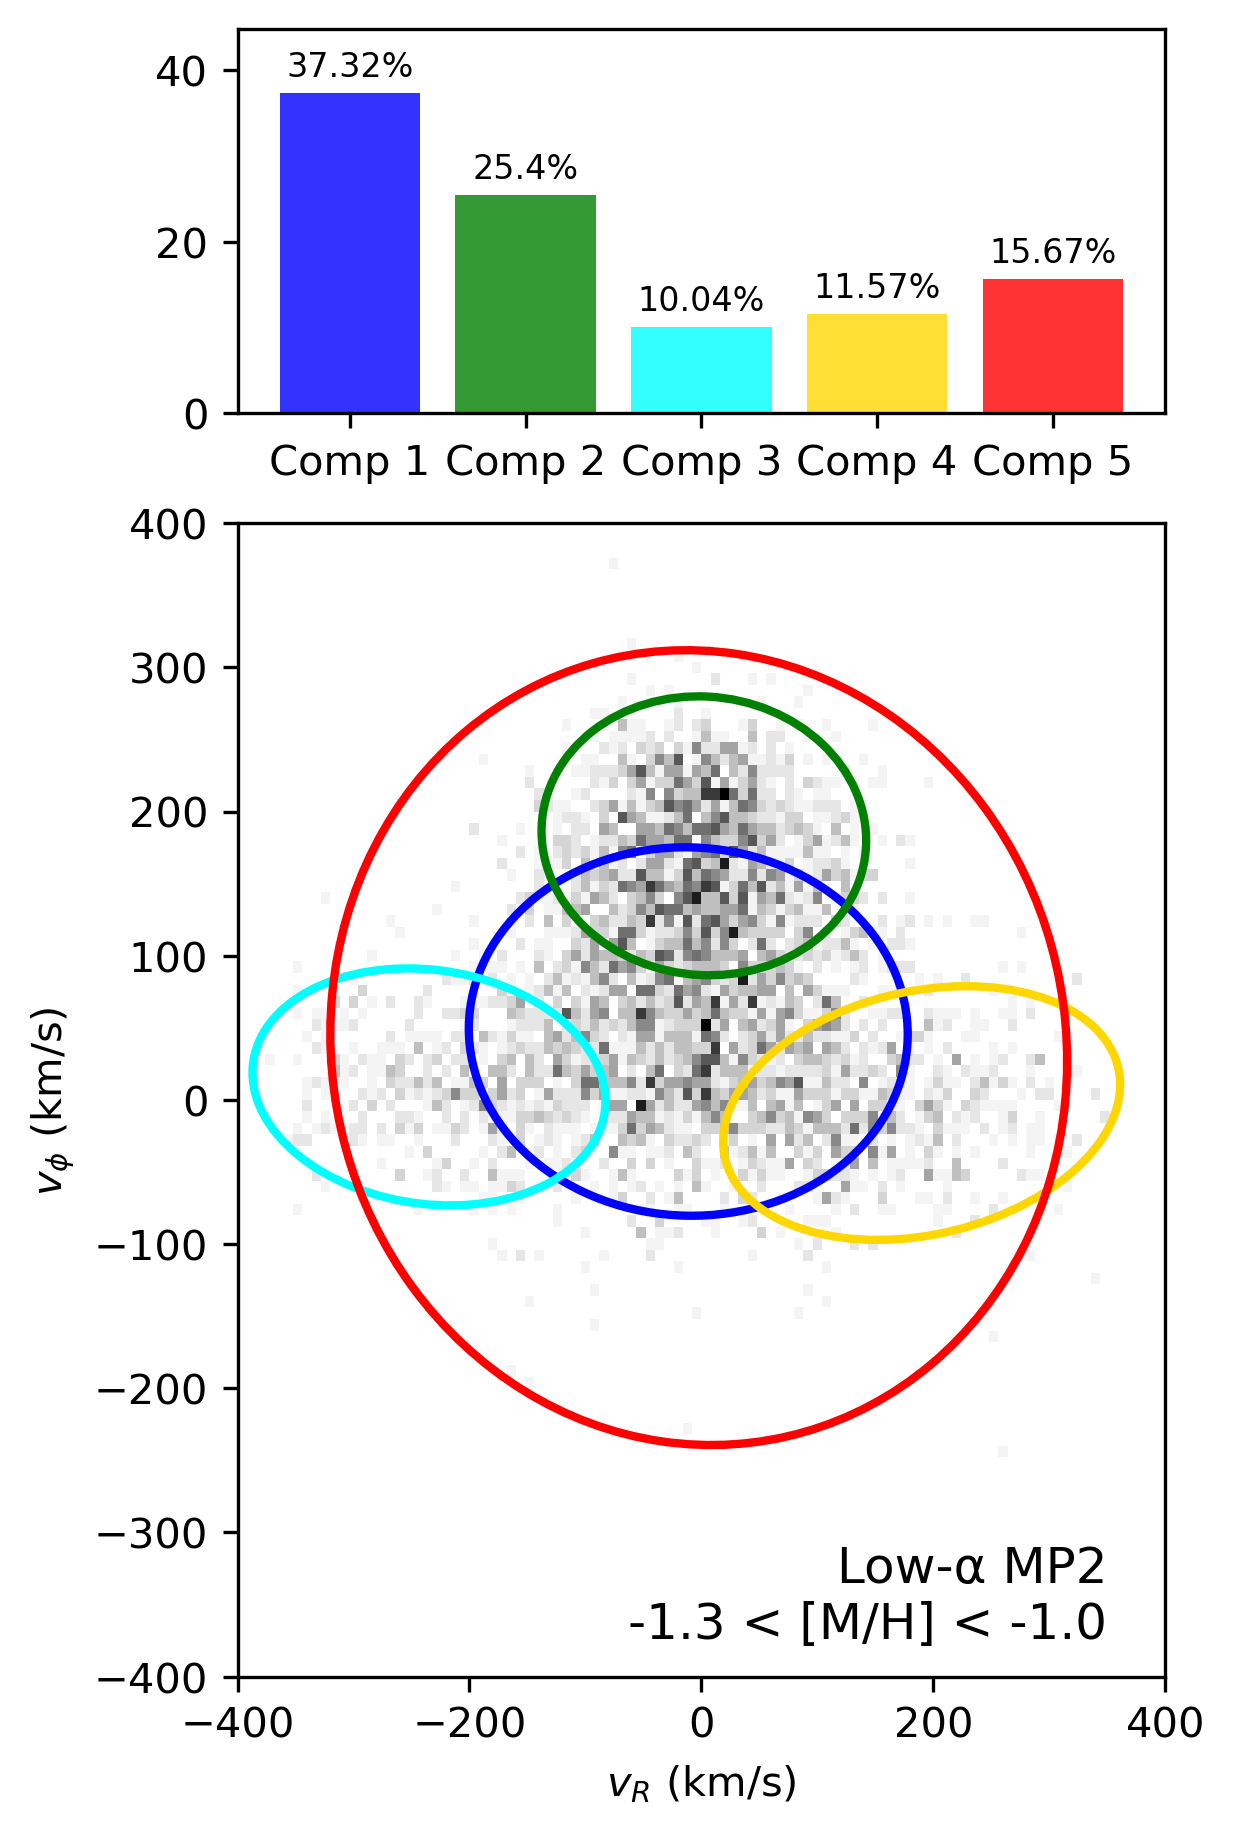
\includegraphics[width=\linewidth]{../figures/gmm_mp2_low_alpha_k6.png}
    \caption{\href{https://raw.githack.com/raunaq-rai/Disentangling-the-Milky-Way-using-GMM/main/figures/MP2\_low\_\_\_\_-1.3\%5BM\_H\%5D-1.0.html}{MP2 $\alpha_{\mathrm{low}}$}}
    \label{fig:low_mp2}
  \end{subfigure}


  \caption{XD–GMM decomposition across $\alpha$-sequences and metallicity bins. Top row: high-$\alpha$; bottom row: low-$\alpha$.}
  \label{fig:gmm_alpha_bins}
\end{figure}



\section*{Recommendations and Next Steps}

This project confirms the absence of disc-like kinematics below $\mathrm{[M/H]} \sim -2$ 
and finds earlier rotational support in the high $\alpha$ sequence. Future work should move 
beyond Gaussian mixtures, which cannot capture non-Gaussian or asymmetric structures, and 
consider models based on distribution functions. Addressing measurement uncertainties, 
particularly in $\alpha$, will improve sequence classification, especially 
at low metallicities. Incorporating a formal selection function will also allow for global 
population estimates. The unexpected appearance of GS/E-like components in the high $\alpha$ 
sequence requires further investigation, likely reflecting contamination or substructure overlap.

\section*{Conclusion and Research Impact}

We reproduce the key results of Zhang et al.~ \cite{zhang2024existencemetalpoordiscmilky} and 
extend them by separating stars by $\alpha$ abundance. Our findings support a two-phase disc 
formation model, with the high $\alpha$ sequence developing rotation at lower metallicity than 
the low $\alpha$ population. This demonstrates the power of combining chemistry and kinematics to 
trace the Milky Way’s evolution and provides a framework for analysing future survey data.

\newpage{}

993 / 1000 words








\bibliographystyle{unsrt}  
\bibliography{references}

% End of two-column content
\end{multicols}



\end{document}
